% ============================================================================
% Surrogate Models in Economics and Finance (GP toolbox in the appendix)
% Duration: 90 minutes (main part ~45; appendix = reference material)
% ============================================================================

\documentclass[aspectratio=169,11pt]{beamer}

% ---------- Theme and colors ----------
\usecolortheme{dove}
\setbeamertemplate{navigation symbols}{}
\setbeamertemplate{footline}{%
  \hfill\usebeamerfont{page number in head/foot}%
  \usebeamercolor[fg]{normal text}%
  \insertframenumber\,/\,\inserttotalframenumber\kern1em\vskip4pt}
\setbeamerfont{frametitle}{size=\huge}

% ---------- Packages ----------
\usepackage[utf8]{inputenc}
\usepackage[T1]{fontenc}
\usepackage{amsmath,amssymb,amsfonts}
\usepackage{bm}
\usepackage{graphicx}
\usepackage{tikz}
\usetikzlibrary{shapes,arrows.meta,positioning,calc,fit,backgrounds,patterns,decorations.pathreplacing}
\usepackage{pgfplots}
\pgfplotsset{compat=1.18}
\usepackage{booktabs}
\usepackage{hyperref}
\usepackage{multicol}
\usepackage{xcolor}
\usepackage{algorithm}
\usepackage{algorithmic}
\usepackage{listings}
\usepackage{pifont}

% ---------- Listings style for Python ----------
\lstset{
    language=Python,
    basicstyle=\small\ttfamily,
    keywordstyle=\color{uzhblue}\bfseries,
    commentstyle=\color{uzhgreydark}\itshape,
    stringstyle=\color{darkgreen},
    showstringspaces=false,
    breaklines=true,
    frame=none,
    xleftmargin=0pt,
    aboveskip=4pt,
    belowskip=4pt,
    escapeinside={(*@}{@*)},
}

% ---------- Custom colors ----------
\definecolor{uzhblue}{rgb}{0,0,0.5}
\definecolor{uzhgreylight}{RGB}{236,238,241}
\definecolor{uzhgreydark}{RGB}{81,86,94}
\definecolor{harvardcrimson}{RGB}{153,0,0}
\definecolor{unil@blue}{RGB}{0,140,204}
\definecolor{unil@black}{RGB}{35,31,32}
\definecolor{darkgreen}{RGB}{0,100,0}
\definecolor{darkred}{RGB}{139,0,0}
\definecolor{softblue}{RGB}{70,130,180}
\definecolor{softorange}{RGB}{230,159,0}
\definecolor{softgreen}{RGB}{0,158,115}

% ---------- Set beamer colors ----------
\setbeamercolor{frametitle}{bg=uzhgreylight, fg=uzhblue}
\setbeamercolor{title}{fg=uzhblue}
\setbeamercolor{structure}{fg=uzhblue}
\setbeamercolor{block title}{bg=unil@blue, fg=white}
\setbeamercolor{block body}{bg=uzhgreylight}
\setbeamercolor{block title alerted}{bg=darkred,fg=white}
\setbeamercolor{block body alerted}{bg=red!5}
\setbeamercolor{block title example}{bg=darkgreen,fg=white}
\setbeamercolor{block body example}{bg=green!5}
\setbeamercolor{item}{fg=unil@black}
\setbeamercolor{normal text}{fg=unil@black}

% ---------- Emphasis and hyperlinks ----------
\newcommand{\emphc}[1]{\textcolor{harvardcrimson}{#1}}
\hypersetup{colorlinks,linkcolor=harvardcrimson,urlcolor=harvardcrimson}

% ---------- Math commands ----------
\newcommand{\x}{\bm{x}}
\newcommand{\w}{\bm{w}}
\newcommand{\bb}{\bm{b}}
\newcommand{\z}{\bm{z}}
\newcommand{\W}{\bm{W}}
\newcommand{\X}{\bm{X}}
\renewcommand{\a}{\bm{a}}
\newcommand{\R}{\mathbb{R}}
\newcommand{\E}[1]{\mathbb{E}\!\left[#1\right]}
\DeclareMathOperator*{\argmin}{arg\,min}
\DeclareMathOperator*{\argmax}{arg\,max}

% ---------- Callout boxes and accents (lazy-learning frames) ----------
\usepackage[most]{tcolorbox}
\definecolor{stone}{RGB}{120,118,112}
\definecolor{vgold}{RGB}{183,142,55}
\newcommand{\lemph}[1]{{\color{uzhblue}\bfseries #1}}
\newcommand{\gemph}[1]{{\color{vgold!75!black}\bfseries #1}}
\newcommand{\visualcaption}[1]{{\scriptsize\color{stone}\itshape #1}}
\newtcolorbox{pitfall}[1][Pitfall]{%
  colback=harvardcrimson!6,colframe=harvardcrimson,coltitle=white,fonttitle=\bfseries,
  title={#1},rounded corners,boxrule=1pt,left=5pt,right=5pt,top=3pt,bottom=3pt}
\newtcolorbox{recipe}[1][Recipe]{%
  colback=softgreen!7,colframe=softgreen!80!black,coltitle=white,fonttitle=\bfseries,
  title={#1},rounded corners,boxrule=1pt,left=5pt,right=5pt,top=3pt,bottom=3pt}

% ---------- Title ----------
\title[CEMRACS 2026 $\cdot$ Surrogates]
{Computational and AI Methods in Climate Economics}
\subtitle{Lecture 2 (Part 2) --- Surrogate models and Gaussian processes for economics and finance}
\author{Simon Scheidegger}
\institute{HEC Lausanne $\cdot$ Grantham Research Institute, LSE}
\date{July 15, 2026 \,$\cdot$\, CIRM, Marseille, France}

\begin{document}

% --- Exercise pause badge ---
\newcommand{\exercisepause}{%
  \tikz[baseline=(X.base)]{\node[fill=darkgreen!80!black, text=white,
  rounded corners=2pt, inner sep=3pt, font=\scriptsize\bfseries](X){PAUSE --- 5 min};}}
% ============================================================================
% PART 0: TITLE & OUTLINE
% ============================================================================

% --- Slide 1: Title ---
{\setbeamercolor{background canvas}{bg=uzhgreylight}
\begin{frame}
\titlepage
\vspace{-0.4cm}
\begin{center}
{\footnotesize Based on: Chen, Didisheim \& Scheidegger (2026), \emph{J.\ Financial Economics}; Friedl et al.\ (2023); K\"ubler, Scheidegger \& Surbek (2026, forthcoming in \emph{JPE Macroeconomics})}\\[8pt]
{\footnotesize \url{https://cemracs2026.math.cnrs.fr/en/}}
\end{center}
\end{frame}
}

% --- Slide 2: Roadmap ---
\begin{frame}{Roadmap of This Lecture}
\textbf{Main part --- surrogate models in economics and finance:}
\begin{itemize}\itemsep2pt
  \item Why surrogates? From lookup tables to deep neural networks
  \item Pseudo-states: model parameters as extra inputs
  \item Building, validating, and stress-testing a surrogate
  \item Applications: structural estimation, uncertainty quantification, optimal policy, option pricing
  \item A pitfall to know: \emphc{lazy learning} --- and how to fix it
\end{itemize}

\vspace{0.4em}
\textbf{Appendix --- the Gaussian-process toolbox:}
\begin{itemize}\itemsep2pt
  \item GP regression and deep kernels
  \item Bayesian active learning
\end{itemize}

\vspace{0.3em}
\begin{center}
{\scriptsize Hands-on: \texttt{04\_Surrogate\_Primer.ipynb} (main part); notebooks \texttt{05\_GP\_and\_BAL.ipynb} and \texttt{06\_Deep\_Kernel\_Learning.ipynb} accompany the appendix.}
\end{center}
\end{frame}


% --- Learning objectives ---
\begin{frame}{Learning objectives}
\textbf{By the end of this lecture you should be able to:}
\begin{itemize}
  \item Explain what a surrogate model is and why economics and finance are ideal terrain for them (we own the data-generating model)
  \item Design and train deep surrogates that approximate expensive economic models by treating parameters as pseudo-states
  \item Compare approximation methods (polynomials, sparse grids, GPs, DNNs) and recognize when each is appropriate
  \item Sketch the main use cases: structural estimation, uncertainty quantification, optimal policy design, and option-pricing calibration
  \item Diagnose \emphc{lazy learning} in residual-trained surrogates and apply the anchor/distillation and residual-correction fixes
\end{itemize}
\vspace{0.3em}
{\small The Gaussian-process machinery behind several of these applications (GP regression, active learning) is developed in the \emphc{appendix} and in notebooks \texttt{05\_GP\_and\_BAL.ipynb} and \texttt{06\_Deep\_Kernel\_Learning.ipynb}.}
\end{frame}


% ============================================================================
% PART I: DEEP SURROGATE MODELS
% ============================================================================
\section{Deep Surrogate Models}

% --- Slide 3: Motivation ---
\begin{frame}{Motivation: Why Surrogates?}
\begin{block}{The computational bottleneck}
Economic \& financial models are expensive to evaluate:
\begin{itemize}
  \item Global solutions of dynamic stochastic models (DEQNs)
  \item PDE-based models (HJB, Black--Scholes for exotics)
  \item Monte Carlo simulations for risk measures
\end{itemize}
\end{block}

\vspace{0.3cm}
\begin{alertblock}{Key insight}
\emphc{We know the true model} --- we can generate \emph{unlimited} training data by solving the model on a design of experiments.
\end{alertblock}

\vspace{0.3cm}
\textbf{Goal:} Build a \emphc{surrogate} $\phi(\cdot\,|\,\theta_{NN})$ that approximates $f(\cdot)$ but evaluates \emph{orders of magnitude faster}.
\end{frame}

% --- Slide 4: Look-up Tables to Neural Networks ---
\begin{frame}{Look-up Tables $\to$ Neural Networks}
\begin{columns}[T]
\begin{column}{0.42\textwidth}
\textbf{Traditional:} pre-compute \& interpolate.\\[2pt]
\begin{center}
\footnotesize
\begin{tabular}{cc}
\toprule
$x$ & $\Phi(x)$ \\
\midrule
$-2.0$ & $0.0228$ \\
$-1.0$ & $0.1587$ \\
$\phantom{-}0.0$ & $0.5000$ \\
$\phantom{-}1.0$ & $0.8413$ \\
$\phantom{-}2.0$ & $0.9772$ \\
\bottomrule
\end{tabular}
\end{center}
\vspace{2pt}
{\footnotesize Example: standard normal CDF table.}
\end{column}

\begin{column}{0.55\textwidth}
\textbf{21st-century look-up table:}\\[2pt]
A neural network memorizes $\x \mapsto y$:
\[
\phi(\x_t\,|\,\theta_{NN}) \approx y_t = f(\x_t)
\]
\vspace{-4pt}
\begin{center}
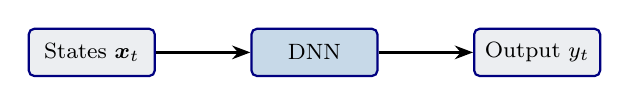
\begin{tikzpicture}[
    mlstep/.style={rectangle, draw=uzhblue, fill=uzhgreylight,
        minimum width=1.6cm, minimum height=0.6cm, font=\footnotesize,
        rounded corners=2pt, thick},
    >=Stealth
]
\node[mlstep] (input) {States $\x_t$};
\node[mlstep, right=1.2cm of input, fill=softblue!30] (dnn) {DNN};
\node[mlstep, right=1.2cm of dnn] (output) {Output $y_t$};
\draw[->, thick] (input) -- (dnn);
\draw[->, thick] (dnn) -- (output);
\end{tikzpicture}
\end{center}
\vspace{2pt}
{\footnotesize \emphc{Continuous}, \emphc{differentiable}, works in \emphc{any dimension}.}
\end{column}
\end{columns}
\end{frame}

% --- Slide 5: Pseudo-States ---
\begin{frame}{Pseudo-States: The Key Idea}
\begin{block}{Core insight (Chen, Didisheim \& Scheidegger 2026)}
Treat model parameters $\theta$ as \emphc{extra state variables}:
\vspace{-2pt}
\[
\tilde{\x} = \bigl(\underbrace{s_1,\dots,s_n}_{\text{states}},\;
\underbrace{\theta_1,\dots,\theta_p}_{\text{parameters}}\bigr)
\in \R^{d}, \quad d = n + p.
\]
\vspace{-6pt}
\end{block}

\vspace{-0.1cm}
\begin{center}
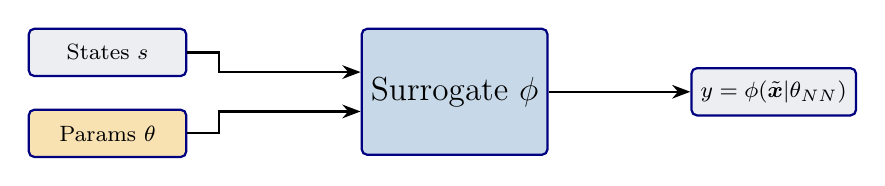
\begin{tikzpicture}[
    mlstep/.style={rectangle, draw=uzhblue, fill=uzhgreylight,
        minimum width=2cm, minimum height=0.6cm, font=\footnotesize,
        rounded corners=2pt, thick},
    >=Stealth
]
\node[mlstep] (states) {States $s$};
\node[mlstep, below=0.4cm of states, fill=softorange!30] (params) {Params $\theta$};

\node[mlstep, right=2.2cm of states, yshift=-0.5cm, fill=softblue!30,
      minimum width=2.2cm, minimum height=1.6cm] (surr) {\large Surrogate $\phi$};

\node[mlstep, right=1.8cm of surr] (output) {$y = \phi(\tilde{\x}|\theta_{NN})$};

\draw[->, thick] (states.east) -- ++(0.4,0) |- ([yshift=0.25cm]surr.west);
\draw[->, thick] (params.east) -- ++(0.4,0) |- ([yshift=-0.25cm]surr.west);
\draw[->, thick] (surr) -- (output);
\end{tikzpicture}
\end{center}

\vspace{0.1cm}
Solve the model \emphc{once} over the full augmented space $\Rightarrow$ instant evaluation for \emph{any} parameter configuration.
\end{frame}

% --- Slide 6: Building the Surrogate ---
\begin{frame}{Building the Surrogate}
\begin{enumerate}
  \item \textbf{Design:} Draw $\tilde{\x}_i$ uniformly from $[\underline{x},\bar{x}]^d$, \quad $i = 1,\dots,m$.
  \item \textbf{Label:} Compute $y_i = f(\tilde{\x}_i)$ using the expensive model.
  \item \textbf{Train:} Minimize the empirical risk:
  \[
  \hat{\theta}_{NN} = \argmin_{\theta_{NN}} \frac{1}{m}\sum_{i=1}^{m}
  \bigl|\phi(\tilde{\x}_i\,|\,\theta_{NN}) - y_i\bigr|^2.
  \]
  \item \textbf{Validate:} On a held-out test set, compute max / mean absolute error.
\end{enumerate}

\vspace{0.4cm}
\begin{block}{Remark}
Since we can generate \emph{unlimited} data from the true model, classical overfitting from data scarcity is not the binding constraint. The binding errors come from \emphc{approximation} (network capacity vs.\ true regularity of $f$) and from \emphc{label noise} when $f$ is itself an approximate inner solver (Euler residuals, Monte Carlo simulation).
\end{block}
\end{frame}

% --- Slide 7: Why Surrogates Are Different ---
\begin{frame}[shrink=4]{Why Surrogates $\neq$ Standard ML}
\begin{columns}[T]
\begin{column}{0.48\textwidth}
\textbf{Standard supervised learning:}
\begin{itemize}
  \item Data is \emph{scarce} and noisy
  \item Overfitting is a major concern
  \item Regularization, early stopping, cross-validation
  \item Small learning rates, careful tuning
\end{itemize}
\end{column}
\begin{column}{0.48\textwidth}
\textbf{Surrogate modeling:}
\begin{itemize}
  \item Data is \emphc{unlimited} (we own the model)
  \item Labels are \emphc{exact} (or noise-free)
  \item Can use large epochs, aggressive LR
  \item Focus on \emph{approximation error}, not generalization
\end{itemize}
\end{column}
\end{columns}

\vspace{0.5cm}
\begin{block}{Once trained}
\begin{itemize}
  \item \emphc{Accurate enough for the downstream task} (relative errors typically $10^{-3}$--$10^{-5}$ on benchmarks; verify per application)
  \item \emphc{Orders of magnitude faster} than the original model
  \item \emphc{Differentiable:} gradients via automatic differentiation (backprop)
\end{itemize}
\end{block}
\end{frame}

% --- Slide 8: Speed Comparison ---
\begin{frame}{Speed Comparison: Option Pricing}
\begin{center}
{\footnotesize From Chen, Didisheim \& Scheidegger (2026), \emph{J.\ Financial Economics}:}

\vspace{0.2cm}
\small
\begin{tabular}{l r r r}
\toprule
\textbf{Task} & \textbf{FFT} & \textbf{Surr.\ (CPU)} & \textbf{Surr.\ (GPU)} \\
\midrule
Single price & $23$ ms & $\emphc{0.03}$ ms & --- \\
1-day calib.\ ($6\!\times\!10^5$) & $3.3$ h & $\emphc{18}$ s & $\emphc{0.4}$ s\\
1-year calib.\ ($1.5\!\times\!10^8$) & ${\approx}\,100$ d & $\emphc{1.2}$ h & $\emphc{98}$ s\\
\bottomrule
\end{tabular}
\end{center}

\vspace{0.3cm}
\begin{alertblock}{Takeaway}
Deep surrogates enable \emphc{real-time calibration} of option pricing models --- tasks that previously took days or were infeasible.
\end{alertblock}
\end{frame}

% --- Slide 9: Comparison of Approximation Methods ---
\begin{frame}{Comparison of Approximation Methods}
\begin{center}
\small
\begin{tabular}{l c c c c}
\toprule
\textbf{Criterion} & \textbf{Polynomials/Splines} & \textbf{Sparse Grids} & \textbf{GPs} & \textbf{DNNs} \\
\midrule
High raw dim.\ ($d > 10$, no AS) & \textcolor{darkred}{\ding{55}} & \textcolor{softorange}{$\sim$} & \textcolor{darkred}{\ding{55}} & \textcolor{darkgreen}{\ding{51}} \\
Local features / kinks    & \textcolor{darkred}{\ding{55}} & \textcolor{darkgreen}{\ding{51}} & \textcolor{softorange}{$\sim$} & \textcolor{darkgreen}{\ding{51}} \\
Irregular domains          & \textcolor{darkred}{\ding{55}} & \textcolor{darkred}{\ding{55}} & \textcolor{darkgreen}{\ding{51}} & \textcolor{darkgreen}{\ding{51}} \\
Large training set ($N > 10^4$) & \textcolor{darkgreen}{\ding{51}} & \textcolor{softorange}{$\sim$} & \textcolor{darkred}{\ding{55}} & \textcolor{darkgreen}{\ding{51}} \\
Built-in uncertainty & \textcolor{darkred}{\ding{55}} & \textcolor{darkred}{\ding{55}} & \textcolor{darkgreen}{\ding{51}} & \textcolor{darkred}{\ding{55}} \\
\bottomrule
\end{tabular}
\end{center}

\vspace{0.3cm}
\begin{itemize}
  \item \textbf{DNNs} excel in high dimensions with large data.
  \item \textbf{GPs} provide \emphc{built-in uncertainty quantification} --- crucial for active learning and Bayesian inference.
  \item \textbf{Combining both} (GP for moderate $d$ with UQ, DNN for high $d$) is a powerful strategy.
\end{itemize}
\end{frame}

% --- Slide 10: Application I — Structural Estimation ---
\begin{frame}{Application I: Structural Estimation}
\small
\textbf{Goal:} Estimate structural parameters $\theta$ from data via SMM:
\[
\hat{\theta}_{SMM} = \argmin_\theta\; [m(\theta)-\hat{m}^{\mathrm{data}}]^\top \, W \, [m(\theta)-\hat{m}^{\mathrm{data}}],
\]
where $m(\theta)$ are model-implied moments and computing them naively requires solving and simulating the model for each candidate $\theta$.

\vspace{0.15cm}
\begin{block}{Surrogate-based estimation}
\begin{enumerate}\itemsep0pt
  \item Train a surrogate policy $\phi(x,\theta)$ over \emphc{states and parameters} (pseudo-states).
  \item Reuse the trained surrogate to simulate moments $m(\theta)$ without re-solving the model.
  \item Evaluate the SMM criterion over many $\theta$ values via grid search or standard optimization.
\end{enumerate}
\end{block}

\vspace{0.15cm}
\textbf{Result:} Repeated SMM evaluations in \emphc{seconds} instead of weeks.\\
(Chen, Didisheim \& Scheidegger 2026)
\end{frame}

% --- Slide 11: Application II — Uncertainty Quantification ---
\begin{frame}{Application II: Uncertainty Quantification}
\textbf{DeepUQ} (Friedl, K\"ubler, Scheidegger \& Usui 2023):

\vspace{0.3cm}
\begin{center}
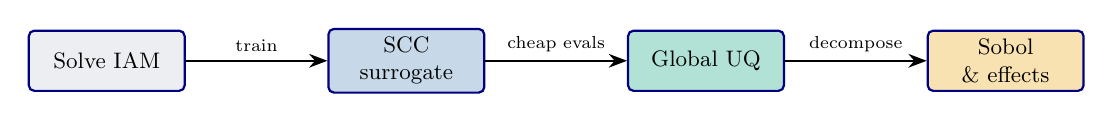
\begin{tikzpicture}[
    mlstep/.style={rectangle, draw=uzhblue, fill=uzhgreylight,
        minimum width=2.2cm, minimum height=0.85cm, font=\small,
        rounded corners=2pt, thick, align=center},
    >=Stealth, scale=0.9, transform shape
]
\node[mlstep] (model) {Solve IAM};
\node[mlstep, right=2.0cm of model, fill=softblue!30] (surr) {SCC\\surrogate};
\node[mlstep, right=2.0cm of surr, fill=softgreen!30] (uq) {Global UQ};
\node[mlstep, right=2.0cm of uq, fill=softorange!30] (out) {Sobol\\\& effects};

\draw[->, thick] (model) -- node[midway, above, font=\scriptsize]{train} (surr);
\draw[->, thick] (surr) -- node[midway, above, font=\scriptsize]{cheap evals} (uq);
\draw[->, thick] (uq) -- node[midway, above, font=\scriptsize]{decompose} (out);
\end{tikzpicture}
\end{center}

\vspace{0.2cm}
\begin{itemize}\small\itemsep1pt
  \item Solve a high-dimensional IAM, train a surrogate for the \emphc{social cost of carbon} $\mathrm{SCC}(\theta)$
  \item Cheap surrogate evaluations enable \emphc{global sensitivity analysis}: Sobol indices, univariate effects
  \item Identifies which climate/economic parameters drive SCC uncertainty
\end{itemize}
\end{frame}

% --- Slide 12: Application III — Optimal Policy ---
\begin{frame}{Application III: Optimal Policy}
K\"ubler, Scheidegger \& Surbek (2026, forthcoming in \emph{JPE Macroeconomics}):

\vspace{0.3cm}
\begin{itemize}
  \item High-dimensional integrated assessment model (IAM)
  \item \emphc{GP surrogate + Bayesian Active Learning (BAL)} for the value function
  \item GP provides \emph{uncertainty quantification} at each point
  \item BAL selects training points where uncertainty is highest
  \item Result: optimal carbon tax policy
\end{itemize}

\vspace{0.3cm}
\begin{alertblock}{Preview}
The appendix introduces \emphc{Gaussian Processes} and \emphc{Bayesian Active Learning} --- the tools behind this application, which Lecture 3 covers in depth.
\end{alertblock}
\end{frame}

% --- Slide 12b: Application IV — Implied Volatility Surface ---
\begin{frame}{Application IV: The Implied Volatility Surface}
\textbf{Goal:} Learn the mapping from option characteristics to implied volatility.
\[
\sigma_{IV} = \phi(K, T, S_0, r, \theta_{\text{model}})
\]

\vspace{0.15cm}
\begin{center}
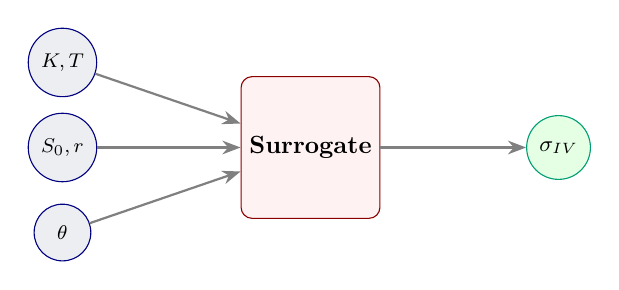
\begin{tikzpicture}[scale=0.9, transform shape,
    node distance=1.8cm,
    input/.style={circle, draw=uzhblue, fill=uzhgreylight, minimum size=0.8cm, font=\footnotesize},
    hidden/.style={rectangle, draw=darkred, fill=red!5, minimum width=1.8cm, minimum height=2cm, rounded corners},
    output/.style={circle, draw=softgreen, fill=green!10, minimum size=0.9cm, font=\small},
    arr/.style={-Stealth, thick, gray}
]
    \node[input] (K) at (0, 1.2) {$K, T$};
    \node[input] (S) at (0, 0) {$S_0, r$};
    \node[input] (P) at (0, -1.2) {$\theta$};
    \node[hidden] (net) at (3.5, 0) {\textbf{Surrogate}};
    \node[output] (IV) at (7, 0) {$\sigma_{IV}$};
    \draw[arr] (K) -- (net);
    \draw[arr] (S) -- (net);
    \draw[arr] (P) -- (net);
    \draw[arr] (net) -- (IV);
\end{tikzpicture}
\end{center}

\vspace{0.1cm}
{\footnotesize\textbf{Benefits.}
\begin{itemize}\itemsep0pt
    \item \textbf{Calibration:} fit $\theta$ by gradient descent on $\sum_i [\phi - \sigma_{IV}^{\mathrm{mkt}}]^2$; $\partial\phi/\partial\theta$ from autograd.
    \item \textbf{Arbitrage-free:} differentiable penalties for calendar ($\partial_T C \!\ge\! 0$) and butterfly ($\partial^2_K C \!\ge\! 0$) violations.
    \item \textbf{Speed:} real-time pricing for stochastic-vol models without closed form.
\end{itemize}}
\end{frame}

% --- Slide: Pseudo-States — Policy Parameterization ---
\begin{frame}{Pseudo-States: Policy Parameterization}
\begin{block}{Split the parameter vector}
\small
$\theta = (\theta_{\text{model}}, \theta_{\text{pol}})$: \emphc{model} = environment (preferences, technology); \emphc{policy} = decision rule (tax path, Taylor coefficients). Both go in as pseudo-state; optimise by autograd through $\phi$:
\vspace{-4pt}
\[
\theta_{\text{pol}}^*(\theta_{\text{model}}) = \argmax_{\theta_{\text{pol}}} \;\phi\bigl(s,\, \theta_{\text{model}},\, \theta_{\text{pol}}\bigr)
\]
\vspace{-6pt}
\end{block}

\vspace{0.1cm}
\begin{columns}[T]
\begin{column}{0.48\textwidth}
\begin{exampleblock}{Carbon tax}
\begin{itemize}\setlength{\itemsep}{0pt}
  \item Policy: tax trajectory $\theta_{\text{pol}}$
  \item Model: climate sensitivity $\theta_{\text{model}}$
  \item Optimal tax for each $\theta_{\text{model}}$
\end{itemize}
\end{exampleblock}
\end{column}
\begin{column}{0.48\textwidth}
\begin{exampleblock}{Monetary policy}
\begin{itemize}\setlength{\itemsep}{0pt}
  \item Policy: Taylor rule coefficients
  \item Model: preference / technology shocks
  \item Optimal rule via gradient descent
\end{itemize}
\end{exampleblock}
\end{column}
\end{columns}

\vspace{0.15cm}
\emphc{Key:} evaluate welfare for \emph{any} model + policy configuration instantly $\Rightarrow$ no re-solving.
\end{frame}

% --- Slide 14: Practical Tips ---
\begin{frame}{Practical Tips for Surrogate Training}
\begin{columns}[T]
\begin{column}{0.48\textwidth}
\begin{block}{Architecture}
\begin{itemize}\setlength{\itemsep}{1pt}
  \item Swish activation ($x \cdot \sigma(x)$)
  \item 3--5 hidden layers, 128--512 neurons
  \item Linear output (no activation)
\end{itemize}
\end{block}

\begin{block}{Training}
\begin{itemize}\setlength{\itemsep}{1pt}
  \item $m \geq 10^5$ samples (cheap to generate)
  \item Adam, LR $10^{-3}$, reduce on plateau
  \item Hundreds of epochs (no overfit risk)
\end{itemize}
\end{block}
\end{column}

\begin{column}{0.48\textwidth}
\begin{block}{Validation}
\begin{itemize}\setlength{\itemsep}{1pt}
  \item Held-out test set
  \item Max / mean absolute error, $R^2$
  \item Scatter: prediction vs.\ truth
\end{itemize}
\end{block}

\begin{block}{Loss functions}
\begin{itemize}\setlength{\itemsep}{1pt}
  \item MSE: $\frac{1}{m}\sum_i (\phi_i - y_i)^2$
  \item Relative $L^1$: $\frac{1}{m}\sum_i |(\phi_i - y_i)/y_i|$
\end{itemize}
\end{block}
\end{column}
\end{columns}
\end{frame}

% ============================================================================
% PITFALL: LAZY LEARNING
% ============================================================================

% --- Slide: Lazy learning (symptom) ---
\begin{frame}[shrink=10]{Pitfall: Lazy Learning --- Low Residual, Wrong Policy}
\begin{columns}[T,onlytextwidth]
\column{0.46\textwidth}
{\footnotesize
\begin{itemize}\setlength\itemsep{2pt}
  \item \textbf{\color{uzhblue}Symptom.} Lazy training is a \lemph{typical pitfall of unsupervised} (residual-only) learning (Chizat, Oyallon \& Bach, 2019).
  \item It drives the training residual down while the policy stays inaccurate across the state--parameter domain.
\end{itemize}}
\vspace{0.3em}
\begin{itemize}\setlength\itemsep{3pt}\footnotesize
  \item Fix a state, and vary a \emph{parameter} $\theta$ (a taste, a tax, a shock size).
  \item The true policy moves with $\theta$; the lazy surrogate stays \emph{flat}, so it gets the level right on average but the \lemph{sensitivity} wrong.
\end{itemize}
\begin{pitfall}[Too flat in the parameter]
\footnotesize Low loss, weak parameter dependence: the surrogate is convincing only on average.
\end{pitfall}
\column{0.52\textwidth}
\centering
\begin{tikzpicture}
\begin{axis}[width=\linewidth,height=0.52\textheight,
   xlabel={parameter $\theta$},ylabel={policy $g$ at a fixed state},
   xlabel style={font=\scriptsize},ylabel style={font=\scriptsize},
   tick label style={font=\tiny},
   xmin=0,xmax=1,ymin=0,ymax=1.3,
   axis lines=left, clip=false]
 % true: strong dependence on the parameter
 \addplot[uzhblue,very thick,domain=0:1,samples=60]{0.12+0.62*x+0.22*x*x};
 \node[uzhblue,font=\scriptsize\bfseries,anchor=east]
   at (axis cs:0.98,1.04){true $g^\star(\theta)$};
 % lazy surrogate: nearly flat in the parameter
 \addplot[harvardcrimson,very thick,densely dashed,domain=0:1,samples=2]{0.50+0.04*x};
 \node[harvardcrimson,font=\scriptsize\bfseries,anchor=north east]
   at (axis cs:0.97,0.47){lazy $\mathcal{N}(\theta)$};
 % the missed sensitivity, shown as a gap at a large theta
 \draw[<->,thick,stone] (axis cs:0.85,0.55) -- (axis cs:0.85,0.79);
 \node[stone,font=\tiny,anchor=south] at (axis cs:0.55,1.14){missed $\theta$-dependence};
\end{axis}
\end{tikzpicture}\\[1pt]
\visualcaption{At a fixed state, the true policy varies with $\theta$ (blue); the lazy surrogate is almost flat (red dashed), so it misses how the answer should respond to the parameter.}
\end{columns}
\end{frame}

% --- Slide: Lazy learning (the fix) ---
\begin{frame}[shrink=10]{The Fix: Anchors and Distillation}
\vspace*{\fill}
\begin{columns}[T,onlytextwidth]
\column{0.56\textwidth}
\begin{itemize}\setlength\itemsep{2pt}
  \item \textbf{\color{uzhblue}Fix.} Augment the self-supervised residual loss with a small \lemph{semi-supervised distillation} term (Hinton et al., 2015) on a few trusted anchor states:
\end{itemize}
\[
  \ell^{\mathrm{dist}}=\ell
   +\lambda\!\sum_{\x_a\in\mathcal{A}}\!\bigl\|\mathcal{N}(\x_a)-p^\star(\x_a)\bigr\|^2 .
\]
{\footnotesize
\begin{itemize}\setlength\itemsep{2pt}
  \item $\mathcal{A}$: a handful of anchor states.
  \item $p^\star$: reference policies from an accurate solver (perturbation, a low-dimensional solve, or a converged reference run).
\end{itemize}}
\column{0.40\textwidth}
\begin{recipe}[Remedy]
\footnotesize In the deep-UQ application of Friedl et al.\ (2023) --- revisited in Lecture 3 --- only \gemph{10--20 anchors} stabilize training, with leave-one-out agreement \gemph{within $1\%$}.
\end{recipe}
\end{columns}
\vspace*{\fill}
\end{frame}

% --- Slide: Residual learning ---
\begin{frame}[shrink=10]{Residual Learning: Freeze and Correct}
\begin{columns}[T,onlytextwidth]
\column{0.50\textwidth}
\textbf{Idea.} Don't ask the network for the \emph{whole} solution. Ask for the \lemph{correction} to a cheap baseline:
\[
  g(\x)=\underbrace{g_0(\x)}_{\text{frozen guess}}
   +\;\mathcal{N}(\x).
\]
\begin{itemize}\setlength\itemsep{2pt}\footnotesize
  \item $g_0$: a cheap guess, steady state, perturbation, or certainty equivalent.
  \item The net learns only the \emph{small, nonlinear} residual, so \lemph{spectral bias bites far less} (He et al., 2016).
  \item Sane from iteration zero, natural for PDE / HJB, and it scales: disaster planning in production networks (Carvalho et al., 2025).
\end{itemize}
\vspace{0.3em}
{\footnotesize $\rightarrow$ \lemph{The network is a proofreader, not an author.}}
\column{0.48\textwidth}
\centering
\begin{tikzpicture}
\begin{axis}[width=\linewidth,height=0.50\textheight,
   xlabel={\scriptsize state},xmin=0,xmax=3,ymin=-0.5,ymax=2.7,
   tick label style={font=\tiny},label style={font=\scriptsize},
   axis line style={stone},ytick=\empty,
   legend style={font=\tiny,draw=stone!40,at={(0.02,0.98)},
                 anchor=north west,row sep=-1pt}]
  \addplot[stone,thick,dashed,domain=0:3,samples=40]{0.6*x+0.45};
  \addlegendentry{frozen $g_0$ (perturbation)}
  \addplot[harvardcrimson,very thick,domain=0:3,samples=160]
    {0.6*x+0.45+0.30*sin(deg(110*x))};
  \addlegendentry{true policy}
  \addplot[softgreen!80!black,very thick,domain=0:3,samples=160]
    {0.30*sin(deg(110*x))};
  \addlegendentry{$\mathcal{N}$: the correction}
\end{axis}
\end{tikzpicture}\\[2pt]
\visualcaption{The net only fits the small wiggle: frozen guess plus learned correction.}
\end{columns}
\end{frame}

% --- Slide: Summary of the main part ---
\begin{frame}{Summary: Deep Surrogate Models}
\begin{enumerate}
  \item \textbf{Surrogates} = cheap, accurate replicas of expensive models.
  \item \textbf{Pseudo-states} ($\theta$ as extra inputs) unlock:
  \begin{itemize}
    \item Structural estimation (SMM in seconds)
    \item Uncertainty quantification (Sobol indices, univariate effects)
    \item Optimal policy design
  \end{itemize}
  \item \textbf{Key advantage:} unlimited training data $\Rightarrow$ classical overfitting is not the binding constraint.
  \item \textbf{Speed:} orders of magnitude faster than original model.
  \item \textbf{Watch out:} residual-only training can go \emphc{lazy} --- flat in the parameters despite a low loss; anchor it with a few trusted reference solutions.
\end{enumerate}

\vspace{0.3cm}
\begin{block}{Hands-on}
\textbf{Notebook:} \texttt{04\_Surrogate\_Primer.ipynb} --- Black--Scholes surrogate with implied volatility inversion.
\end{block}
\end{frame}

% --- Closing / handoff ---
\begin{frame}{}
\begin{columns}[c]
\column{0.45\textwidth}
\begin{center}
{\Huge \textcolor{uzhblue}{\textbf{Questions?}}}

\vspace{1.0cm}
{\large Simon Scheidegger}\\[4pt]
{\small HEC Lausanne $\cdot$ Grantham Research Institute, LSE}\\[4pt]
\url{https://sischei.github.io}

\vspace{0.6cm}
{\small Materials:~~\url{https://github.com/sischei/cemracs2026_DEQN}}
\end{center}

\column{0.45\textwidth}
\begin{center}
\textbf{Next up:}\\[6pt]
{\large Structural Estimation with SMM}\\[10pt]
{\small The \emphc{estimate} operator, pointed at today's surrogate.}\\[12pt]
{\footnotesize The following appendix collects the Gaussian-process toolbox used across today's applications.}
\end{center}
\end{columns}
\end{frame}


% ============================================================================
% APPENDIX: THE GAUSSIAN-PROCESS TOOLBOX
% ============================================================================
\appendix

{\setbeamercolor{background canvas}{bg=uzhblue}
\setbeamercolor{normal text}{fg=white}
\usebeamercolor[fg]{normal text}
\begin{frame}[plain,c]
\begin{center}
{\Huge\bfseries Appendix}\\[0.4cm]
{\LARGE The Gaussian-Process Toolbox}\\[0.6cm]
{\normalsize A: GP regression \& deep kernels \,$\cdot$\, B: Bayesian active learning}
\end{center}
\end{frame}
}

% ============================================================================
% APPENDIX A: GAUSSIAN PROCESS REGRESSION
% ============================================================================
\section{Appendix A: Gaussian Process Regression}

% --- Slide 16: Why Gaussian Processes? ---
\begin{frame}{Why Gaussian Processes?}
\begin{itemize}
  \item \textbf{Nonparametric:} No fixed architecture; the model grows with data.
  \item \textbf{Built-in uncertainty quantification:} Posterior mean \emph{and} variance at every point.
  \item \textbf{Principled kernel selection:} Encode prior beliefs about smoothness, periodicity, etc.
  \item \textbf{Hyperparameter learning:} Marginal likelihood provides a principled objective.
\end{itemize}

\vspace{0.3cm}
\begin{alertblock}{Complementary to DNNs}
\begin{itemize}
  \item GPs: best for moderate dimensions ($d \leq 10$) with built-in UQ.
  \item DNNs: best for high dimensions ($d \gg 10$) with large data.
  \item Combining both is a powerful strategy (cf.\ the comparison table in the main part).
\end{itemize}
\end{alertblock}

\vspace{0.15cm}
{\tiny \textbf{Foundations:} Rasmussen \& Williams (2006); MacKay (1992); Krause, Singh \& Guestrin (2008).
\textbf{In DP:} Engel, Mannor \& Meir (2005); Deisenroth, Rasmussen \& Peters (2009).
\textbf{Sparse / scalable:} Titsias (2009); Hensman, Fusi \& Lawrence (2013).}
\end{frame}

% --- Foundational slides ---
\begin{frame}{Recall: Multivariate Gaussians}
\begin{columns}[T]
\begin{column}{0.45\textwidth}
A random vector $\bm{x} \in \R^d$ is \emphc{multivariate Gaussian} if
\[
\bm{x} \sim \mathcal{N}(\bm{\mu}, \Sigma)
\]
with density
{\small
\[
p(\bm{x}) \propto
\exp\!\Bigl(-\tfrac{1}{2}(\bm{x}\!-\!\bm{\mu})^\top \Sigma^{-1}(\bm{x}\!-\!\bm{\mu})\Bigr)
\]
}

\vspace{0.2cm}
\begin{block}{Key fact}
A multivariate Gaussian is \emphc{fully characterized} by its mean vector $\bm{\mu}$ and covariance matrix $\Sigma$.
\end{block}
\end{column}

\begin{column}{0.52\textwidth}
\begin{center}
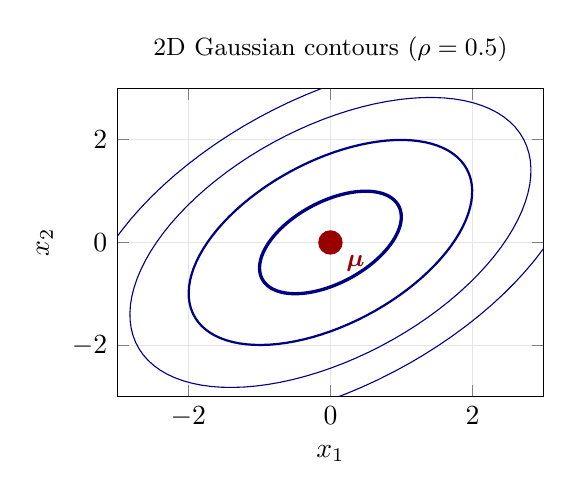
\begin{tikzpicture}
\begin{axis}[
    width=7cm, height=5.5cm,
    xlabel={$x_1$}, ylabel={$x_2$},
    xmin=-3, xmax=3, ymin=-3, ymax=3,
    grid=major, grid style={gray!20},
    every axis plot/.append style={no markers},
    title={\small 2D Gaussian contours ($\rho=0.5$)},
]
\addplot[uzhblue, very thick, domain=0:360, samples=100]
    ({0.707*(1.22*cos(x) - 0.707*sin(x))}, {0.707*(1.22*cos(x) + 0.707*sin(x))});
\addplot[uzhblue, thick, domain=0:360, samples=100]
    ({1.414*(1.22*cos(x) - 0.707*sin(x))}, {1.414*(1.22*cos(x) + 0.707*sin(x))});
\addplot[uzhblue, domain=0:360, samples=100]
    ({2.0*(1.22*cos(x) - 0.707*sin(x))}, {2.0*(1.22*cos(x) + 0.707*sin(x))});
\addplot[uzhblue, thin, domain=0:360, samples=100]
    ({2.5*(1.22*cos(x) - 0.707*sin(x))}, {2.5*(1.22*cos(x) + 0.707*sin(x))});
\addplot[only marks, mark=+, mark size=4pt, harvardcrimson, thick] coordinates {(0,0)};
\node[font=\small, harvardcrimson] at (axis cs:0.35,-0.4) {$\bm{\mu}$};
\end{axis}
\end{tikzpicture}
\end{center}
\end{column}
\end{columns}
\end{frame}

\begin{frame}{Joint and Conditional Distributions}
\begin{columns}[T]
\begin{column}{0.48\textwidth}
\textbf{Joint distribution:}
\[
\begin{pmatrix} x_1 \\ x_2 \end{pmatrix}
\sim \mathcal{N}\!\left(
\begin{pmatrix} \mu_1 \\ \mu_2 \end{pmatrix},
\begin{pmatrix} \Sigma_{11} & \Sigma_{12} \\ \Sigma_{21} & \Sigma_{22} \end{pmatrix}
\right)
\]

\vspace{0.3cm}
\textbf{Conditional distribution:}
\begin{align*}
\mu_{1|2} &= \mu_1 + \Sigma_{12}\Sigma_{22}^{-1}(x_2 - \mu_2)\\
\Sigma_{1|2} &= \Sigma_{11} - \Sigma_{12}\Sigma_{22}^{-1}\Sigma_{21}
\end{align*}

\vspace{0.1cm}
\emphc{This is the mathematical engine behind GP regression.}
\end{column}

\begin{column}{0.50\textwidth}
\begin{center}
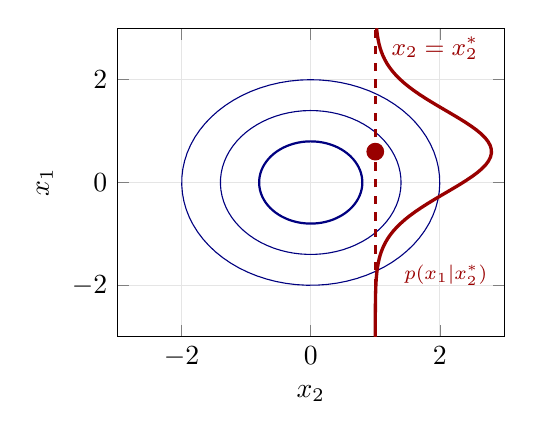
\begin{tikzpicture}
\begin{axis}[
    width=6.5cm, height=5.5cm,
    xlabel={$x_2$}, ylabel={$x_1$},
    xmin=-3, xmax=3, ymin=-3, ymax=3,
    grid=major, grid style={gray!20},
    every axis plot/.append style={no markers},
]
\addplot[uzhblue, thick, domain=0:360, samples=80]
    ({0.8*(0.894*cos(x) - 0.447*sin(x))}, {0.8*(0.447*cos(x) + 0.894*sin(x))});
\addplot[uzhblue, domain=0:360, samples=80]
    ({1.4*(0.894*cos(x) - 0.447*sin(x))}, {1.4*(0.447*cos(x) + 0.894*sin(x))});
\addplot[uzhblue, thin, domain=0:360, samples=80]
    ({2.0*(0.894*cos(x) - 0.447*sin(x))}, {2.0*(0.447*cos(x) + 0.894*sin(x))});
\draw[harvardcrimson, very thick, dashed] (axis cs:1,-3) -- (axis cs:1,3);
\node[font=\small, harvardcrimson, anchor=south west] at (axis cs:1.1,2.2) {$x_2 = x_2^*$};
\addplot[harvardcrimson, very thick, domain=-3:3, samples=80]
    ({1 + 1.8*exp(-(x-0.6)^2/(2*0.64))}, {x});
\node[font=\scriptsize, harvardcrimson, anchor=west, inner sep=1pt]
    at (axis cs:1.4,-1.8) {$p(x_1|x_2^*)$};
\addplot[only marks, mark=*, mark size=3pt, harvardcrimson] coordinates {(1,0.6)};
\end{axis}
\end{tikzpicture}
\end{center}
{\small ``Slicing'' the joint at $x_2 = x_2^*$ yields a 1D Gaussian.}
\end{column}
\end{columns}
\end{frame}

\begin{frame}{From Observations to Interpolation}
\vspace{-0.2cm}
\begin{columns}[T]
\begin{column}{0.38\textwidth}
\begin{center}
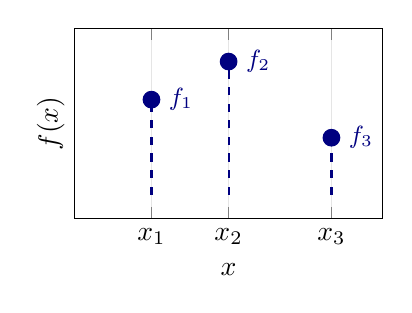
\begin{tikzpicture}
\begin{axis}[
    width=5.5cm, height=4cm,
    xlabel={$x$}, ylabel={$f(x)$},
    xmin=-0.5, xmax=5.5, ymin=-0.5, ymax=3.5,
    grid=major, grid style={gray!20},
    xtick={1,2.5,4.5},
    xticklabels={$x_1$,$x_2$,$x_3$},
    ytick=\empty,
    every axis plot/.append style={no markers},
]
\addplot[uzhblue, thick, dashed] coordinates {(1,0) (1,2.0)};
\addplot[uzhblue, thick, dashed] coordinates {(2.5,0) (2.5,2.8)};
\addplot[uzhblue, thick, dashed] coordinates {(4.5,0) (4.5,1.2)};
\addplot[only marks, mark=*, mark size=3pt, uzhblue] coordinates
    {(1,2.0) (2.5,2.8) (4.5,1.2)};
\node[font=\small, uzhblue, anchor=west] at (axis cs:1.15,2.0) {$f_1$};
\node[font=\small, uzhblue, anchor=west] at (axis cs:2.65,2.8) {$f_2$};
\node[font=\small, uzhblue, anchor=west] at (axis cs:4.65,1.2) {$f_3$};
\end{axis}
\end{tikzpicture}
\end{center}
\end{column}

\begin{column}{0.60\textwidth}
\textbf{Assume} function values are jointly Gaussian:
\vspace{-0.2cm}
{\small
\[
\begin{pmatrix} f_1 \\ f_2 \\ f_3 \end{pmatrix}
\sim \mathcal{N}\!\left(
\bm{0},\;
\begin{pmatrix} K_{11} & K_{12} & K_{13} \\ K_{21} & K_{22} & K_{23} \\ K_{31} & K_{32} & K_{33} \end{pmatrix}
\right)
\]
}

\vspace{-0.1cm}
\emphc{Nearby points ($f_1, f_2$) should be more correlated than distant ones ($f_1, f_3$).}

\vspace{0.1cm}
\textbf{Example} (SE kernel, $\ell = 2$):\;
$K \!=\! \bigl(\begin{smallmatrix} 1.00 & 0.76 & 0.22 \\ 0.76 & 1.00 & 0.61 \\ 0.22 & 0.61 & 1.00 \end{smallmatrix}\bigr)$

\vspace{0.15cm}
Covariance via a \emphc{kernel function}: $K_{ij} = k(x_i, x_j)$

\vspace{0.1cm}
{\small $\Rightarrow$ The kernel encodes our prior belief about function smoothness.}
\end{column}
\end{columns}
\end{frame}

% --- GP — A Distribution Over Functions ---
\begin{frame}{GP: A Distribution Over Functions}
\begin{block}{Definition}
A \emphc{Gaussian Process} is a collection of random variables, any finite number of which have a joint Gaussian distribution:
\[
f(\x) \sim \mathcal{GP}\bigl(\mu(\x),\; k(\x, \x')\bigr).
\]
\end{block}

\begin{itemize}
  \item \textbf{Mean function:} $\mu(\x) = \E{f(\x)}$ \quad (often set to $0$).
  \item \textbf{Covariance function (kernel):} $k(\x,\x') = \E{(f(\x)-\mu(\x))(f(\x')-\mu(\x'))}$.
\end{itemize}

\vspace{0.3cm}
\begin{center}
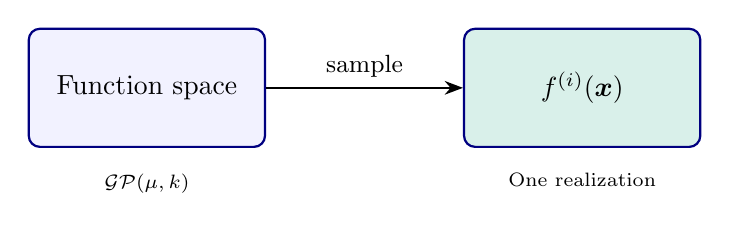
\begin{tikzpicture}[>=Stealth]
\node[draw=uzhblue, thick, rounded corners, fill=blue!5,
      minimum width=3cm, minimum height=1.5cm] (fspace) {Function space};
\node[right=2.5cm of fspace, draw=uzhblue, thick, rounded corners, fill=softgreen!15,
      minimum width=3cm, minimum height=1.5cm] (sample) {$f^{(i)}(\x)$};
\draw[->, thick] (fspace) -- node[above, font=\small]{sample} (sample);
\node[below=0.2cm of fspace, font=\scriptsize] {$\mathcal{GP}(\mu, k)$};
\node[below=0.2cm of sample, font=\scriptsize] {One realization};
\end{tikzpicture}
\end{center}
\end{frame}

% --- Slide 18: The Squared Exponential Kernel ---
\begin{frame}{The Squared Exponential (RBF) Kernel}
\[
k_{SE}(x, x') = \sigma_f^2 \exp\!\left(-\frac{(x - x')^2}{2\ell^2}\right)
\]

\begin{itemize}
  \item $\ell$ = \textbf{length scale} (horizontal correlation range)
  \item $\sigma_f^2$ = \textbf{signal variance} (vertical scale)
\end{itemize}

\vspace{0.2cm}
\begin{center}
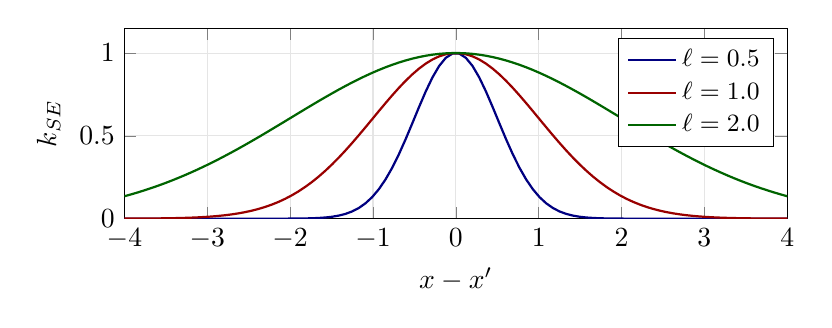
\begin{tikzpicture}
\begin{axis}[
    width=10cm, height=4cm,
    xlabel={$x - x'$}, ylabel={$k_{SE}$},
    xmin=-4, xmax=4, ymin=0, ymax=1.15,
    legend style={at={(0.98,0.95)}, anchor=north east, font=\small},
    grid=major, grid style={gray!20},
    every axis plot/.append style={thick, no markers},
]
\addplot[uzhblue, domain=-4:4, samples=100] {exp(-x^2/(2*0.5^2))};
\addlegendentry{$\ell=0.5$}
\addplot[harvardcrimson, domain=-4:4, samples=100] {exp(-x^2/(2*1.0^2))};
\addlegendentry{$\ell=1.0$}
\addplot[darkgreen, domain=-4:4, samples=100] {exp(-x^2/(2*2.0^2))};
\addlegendentry{$\ell=2.0$}
\end{axis}
\end{tikzpicture}
\end{center}

{\small Larger $\ell$ $\Rightarrow$ smoother functions; smaller $\ell$ $\Rightarrow$ more wiggly.}
\end{frame}

% --- Kernel slides ---
\begin{frame}{The Mat\'ern Kernel Family}
\vspace{-0.2cm}
{\small
$k_{\text{Mat}}(r) = \sigma^2 \frac{2^{1-\nu}}{\Gamma(\nu)}
\bigl(\frac{\sqrt{2\nu}\,r}{\ell}\bigr)^{\!\nu}
K_\nu\!\bigl(\frac{\sqrt{2\nu}\,r}{\ell}\bigr),
\quad r = |x - x'|$}

\vspace{-0.2cm}
\begin{center}
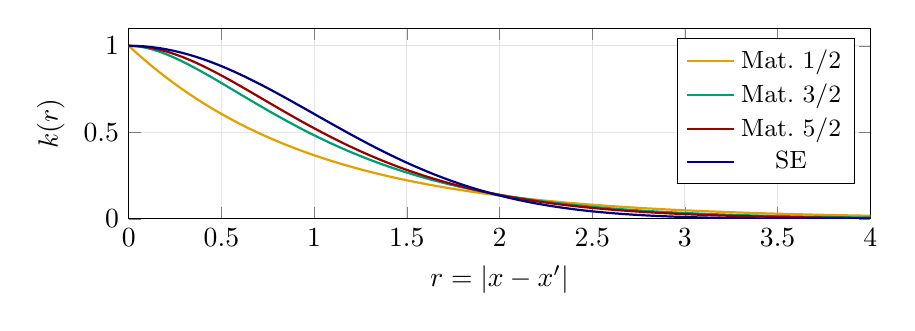
\begin{tikzpicture}
\begin{axis}[
    width=11cm, height=4cm,
    xlabel={$r = |x - x'|$}, ylabel={$k(r)$},
    xmin=0, xmax=4, ymin=0, ymax=1.1,
    grid=major, grid style={gray!20},
    every axis plot/.append style={thick, no markers},
    legend style={at={(0.98,0.95)}, anchor=north east, font=\small},
]
\addplot[softorange, domain=0:4, samples=100] {exp(-x)};
\addlegendentry{Mat.\ 1/2}
\addplot[softgreen, domain=0:4, samples=100] {(1+1.732*x)*exp(-1.732*x)};
\addlegendentry{Mat.\ 3/2}
\addplot[harvardcrimson, domain=0:4, samples=100] {(1+2.236*x+5/3*x^2)*exp(-2.236*x)};
\addlegendentry{Mat.\ 5/2}
\addplot[uzhblue, domain=0:4, samples=100] {exp(-x^2/2)};
\addlegendentry{SE}
\end{axis}
\end{tikzpicture}
\end{center}

\vspace{-0.2cm}
{\small
\begin{itemize}\setlength{\itemsep}{0pt}
  \item $\nu$ controls \emphc{mean-square smoothness}: $\nu\!=\!3/2$ $\Rightarrow$ once MS-differentiable;\; $\nu\!=\!5/2$ $\Rightarrow$ twice;\; SE $\Rightarrow$ $\infty$-smooth.
  \item \textbf{Use case:} Mat\'ern when the true function is \emph{not} infinitely smooth (e.g., has kinks).
\end{itemize}}
\end{frame}

\begin{frame}[shrink=5]{Combining Kernels}
Kernels can be \emphc{added} and \emphc{multiplied} to compose complex priors from simple blocks.

\vspace{0.3cm}
\begin{columns}[T]
\column{0.55\textwidth}
\begin{center}
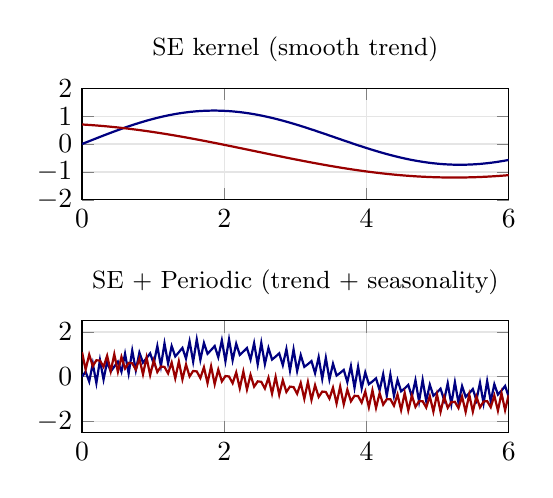
\begin{tikzpicture}
\begin{axis}[
    name=kse,
    width=7cm, height=3cm,
    title={\small SE kernel (smooth trend)},
    xmin=0, xmax=6, ymin=-2, ymax=2,
    grid=major, grid style={gray!20},
    every axis plot/.append style={thick, no markers},
]
\addplot[uzhblue, domain=0:6, samples=80] {sin(deg(0.9*x)) + 0.3*sin(deg(0.4*x))};
\addplot[harvardcrimson, domain=0:6, samples=80] {0.7*cos(deg(0.6*x)) - 0.5*sin(deg(0.3*x))};
\end{axis}

\begin{axis}[
    at={(kse.below south)}, anchor=above north, yshift=-0.3cm,
    width=7cm, height=3cm,
    title={\small SE $+$ Periodic (trend + seasonality)},
    xmin=0, xmax=6, ymin=-2.5, ymax=2.5,
    grid=major, grid style={gray!20},
    every axis plot/.append style={thick, no markers},
]
\addplot[uzhblue, domain=0:6, samples=120]
    {sin(deg(0.9*x)) + 0.3*sin(deg(0.4*x)) + 0.5*sin(deg(180*x))};
\addplot[harvardcrimson, domain=0:6, samples=120]
    {0.7*cos(deg(0.6*x)) - 0.5*sin(deg(0.3*x)) + 0.4*cos(deg(180*x))};
\end{axis}
\end{tikzpicture}
\end{center}

\column{0.42\textwidth}
\begin{block}{Kernel algebra}
\begin{itemize}\setlength{\itemsep}{3pt}
  \item \textbf{$k_1 + k_2$} (OR):\\
  high if \emph{either} is high\\
  $\Rightarrow$ trend + seasonality
  \item \textbf{$k_1 \times k_2$} (AND):\\
  high only if \emph{both} high\\
  $\Rightarrow$ locally periodic
\end{itemize}
\end{block}

\vspace{0.3cm}
{\small \emphc{Compose complex priors} from simple building blocks.}
\end{columns}
\end{frame}

% --- Sampling from the GP Prior ---
\begin{frame}{Sampling from the GP Prior}
\begin{columns}[T]
\begin{column}{0.42\textwidth}
\begin{block}{Algorithm}
\begin{enumerate}\setlength{\itemsep}{1pt}
  \item Grid $x_{1:N}$ over domain
  \item $K_{ij} = k(x_i, x_j)$
  \item Cholesky: $K = LL^\top$
  \item $\bm{f}^{(s)} = L \cdot \bm{u}$, $\bm{u} \sim \mathcal{N}(\bm{0}, I)$
\end{enumerate}
\end{block}
\vspace{0.2cm}
{\small Five functions drawn from a GP prior with SE kernel ($\ell=1$, $\sigma_f=1$).}
\end{column}
\begin{column}{0.56\textwidth}
\begin{center}
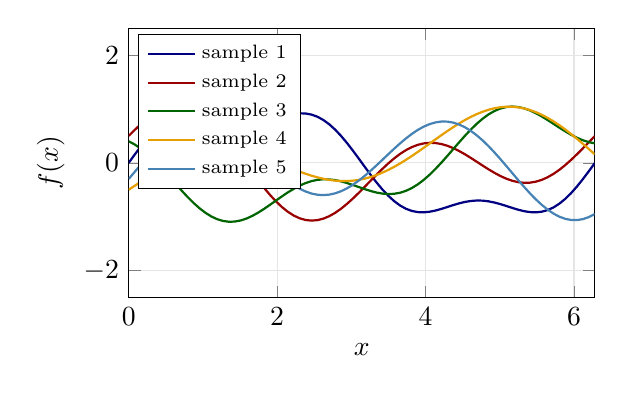
\begin{tikzpicture}
\begin{axis}[
    width=7.5cm, height=5cm,
    xlabel={$x$}, ylabel={$f(x)$},
    xmin=0, xmax=6.28, ymin=-2.5, ymax=2.5,
    grid=major, grid style={gray!20},
    every axis plot/.append style={thick, no markers},
    legend style={at={(0.02,0.98)}, anchor=north west, font=\scriptsize},
]
\addplot[uzhblue, domain=0:6.28, samples=80] {sin(deg(x)) + 0.3*sin(deg(3*x))};
\addlegendentry{sample 1}
\addplot[harvardcrimson, domain=0:6.28, samples=80] {0.5*cos(deg(x)) + 0.7*sin(deg(2*x))};
\addlegendentry{sample 2}
\addplot[darkgreen, domain=0:6.28, samples=80] {-0.8*sin(deg(0.8*x)) + 0.4*cos(deg(2.5*x))};
\addlegendentry{sample 3}
\addplot[softorange, domain=0:6.28, samples=80] {0.6*sin(deg(1.5*x)) - 0.5*cos(deg(0.7*x))};
\addlegendentry{sample 4}
\addplot[softblue, domain=0:6.28, samples=80] {-0.3*cos(deg(1.2*x)) + 0.9*sin(deg(1.8*x))};
\addlegendentry{sample 5}
\end{axis}
\end{tikzpicture}
\end{center}
\end{column}
\end{columns}
\end{frame}

% --- Slide 20: From Prior to Posterior ---
\begin{frame}{From Prior to Posterior: Bayes Rule}
\begin{itemize}
  \item \textbf{Training set:} $\mathcal{D} = \{(\x_i, y_i)\}_{i=1}^n$.
  \item \textbf{Test points:} $\X_*$ where we want predictions.
  \item Joint distribution of training outputs $\bm{f}$ and test outputs $\bm{f}_*$ is Gaussian.
\end{itemize}

\vspace{0.3cm}
\begin{center}
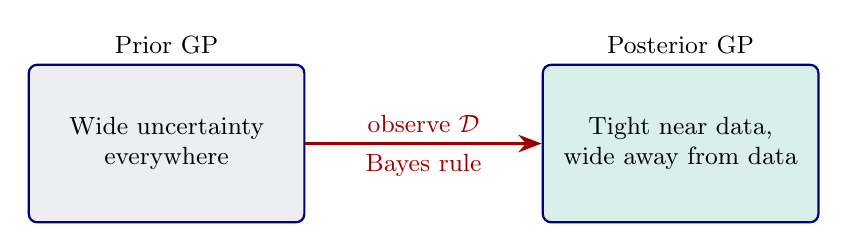
\begin{tikzpicture}[
    mlstep/.style={rectangle, draw=uzhblue, fill=uzhgreylight,
        minimum width=3.5cm, minimum height=2cm, rounded corners=3pt, thick},
    >=Stealth
]
\node[mlstep, label={[font=\small]above:Prior GP}] (prior) {
    \begin{minipage}{3cm}\centering
    \small Wide uncertainty\\everywhere
    \end{minipage}};
\node[mlstep, right=3cm of prior, fill=softgreen!15,
      label={[font=\small]above:Posterior GP}] (post) {
    \begin{minipage}{3cm}\centering
    \small Tight near data,\\wide away from data
    \end{minipage}};
\draw[->, very thick, harvardcrimson] (prior) -- node[above, font=\small]{observe $\mathcal{D}$}
    node[below, font=\small]{\emphc{Bayes rule}} (post);
\end{tikzpicture}
\end{center}

\vspace{0.2cm}
The posterior is \emph{still a GP} --- fully characterized by updated mean and covariance.
\end{frame}

% --- Slide 21: Noiseless GP Regression ---
\begin{frame}{Noiseless GP Regression}
\textbf{Joint distribution:}
\[
\begin{pmatrix} \bm{f} \\ \bm{f}_* \end{pmatrix}
\sim \mathcal{N}\!\left(
\begin{pmatrix} \bm{\mu} \\ \bm{\mu}_* \end{pmatrix},
\begin{pmatrix} K & K_* \\ K_*^\top & K_{**} \end{pmatrix}
\right)
\]

where $K_{ij} = k(\x_i, \x_j)$, \; $(K_*)_{ij} = k(\x_i, \x_*^{(j)})$, \; $(K_{**})_{ij} = k(\x_*^{(i)}, \x_*^{(j)})$.

\vspace{0.3cm}
\textbf{Posterior} (conditioning on $\bm{f}$):
\begin{align}
\bm{\mu}_{*|\mathcal{D}} &= K_*^\top K^{-1}(\bm{f} - \bm{\mu}) + \bm{\mu}_* \label{eq:gp_mean}\\
\Sigma_{*|\mathcal{D}} &= K_{**} - K_*^\top K^{-1} K_* \label{eq:gp_var}
\end{align}

\vspace{0.2cm}
\begin{alertblock}{Key insight}
\begin{itemize}
  \item Near observed data: $K_*^\top K^{-1} K_* \approx K_{**}$ $\Rightarrow$ \emphc{small variance}.
  \item Far from data: $K_*^\top K^{-1} K_* \approx 0$ $\Rightarrow$ \emphc{large variance} (reverts to prior).
\end{itemize}
\end{alertblock}
\end{frame}

% --- Slide 22: Prediction at a Single Test Point ---
\begin{frame}{Prediction at a Single Test Point}
\small
\textbf{Noiseless setting} ($\sigma_y^2 \to 0$ limit; GP interpolates training data). For a single test input $\x_*$:
\vspace{-4pt}
\begin{align}
\bar{f}_* &= \bm{k}_*^\top K^{-1} \bm{f} = \sum_{i=1}^{N} \alpha_i \, k(\x_i, \x_*) \\
\sigma_*^2 &= k(\x_*, \x_*) - \bm{k}_*^\top K^{-1} \bm{k}_*
\end{align}
\vspace{-12pt}

where $\bm{\alpha} = K^{-1}\bm{f}$, $\bm{k}_* = (k(\x_1, \x_*), \dots, k(\x_N, \x_*))^\top$. Noisy form ($K \to K + \sigma_y^2 I$) on next slide.

\begin{block}{Interpretation}
Posterior mean is a \emphc{weighted sum of kernel basis functions} centered at training points:
\vspace{-4pt}
\[
\bar{f}_* = \sum_{i=1}^N \alpha_i \, k(\x_i, \x_*)
\]
\vspace{-10pt}

Each observation $\x_i$ ``pulls'' the prediction via its kernel similarity to $\x_*$.
\end{block}
\end{frame}

% --- Slide 23: GPR with Noisy Data ---
\begin{frame}{GP Regression with Noisy Observations}
\textbf{Observation model:}
\[
y = f(\x) + \varepsilon, \qquad \varepsilon \sim \mathcal{N}(0, \sigma_y^2)
\]

\vspace{0.2cm}
The covariance of \emph{observations} becomes:
\[
\text{cov}[y_p, y_q] = k(\x_p, \x_q) + \sigma_y^2 \delta_{pq}
\]

\vspace{0.2cm}
In matrix form: replace $K$ with
\[
K_y = K + \sigma_y^2 I
\]

\vspace{0.3cm}
\begin{block}{Effect of noise}
\begin{itemize}
  \item Predictions no longer interpolate the data exactly.
  \item Even at training points, there is \emphc{residual uncertainty}.
  \item The noise term $\sigma_y^2 I$ also acts as \emphc{numerical regularization} (``nugget'' / ``jitter'').
\end{itemize}
\end{block}
\end{frame}

% --- Slide 24: Noisy GPR Posterior ---
\begin{frame}{Noisy GPR: Posterior Equations}
\textbf{Posterior mean and variance with noise:}
\begin{align}
\bar{f}_* &= \bm{k}_*^\top (K + \sigma_y^2 I)^{-1} \bm{y} \\
\sigma_*^2 &= k(\x_*, \x_*) - \bm{k}_*^\top (K + \sigma_y^2 I)^{-1} \bm{k}_*
\end{align}

\vspace{0.3cm}
\begin{columns}[T]
\begin{column}{0.48\textwidth}
\textbf{Noiseless} ($\sigma_y^2 = 0$):
\begin{itemize}
  \item Interpolates training points exactly
  \item Variance = 0 at training inputs
  \item Requires $K$ to be positive definite
\end{itemize}
\end{column}
\begin{column}{0.48\textwidth}
\textbf{Noisy} ($\sigma_y^2 > 0$):
\begin{itemize}
  \item Smooths through training points
  \item Variance $> 0$ everywhere
  \item Better numerical conditioning
\end{itemize}
\end{column}
\end{columns}

\vspace{0.3cm}
{\small \textbf{In practice:} Even for noiseless surrogates, adding a small jitter $\sigma_y^2 \sim 10^{-6}$ improves numerical stability.}
\end{frame}

% --- Slide 25: Effect of Kernel Parameters ---
\begin{frame}[shrink=20]{The Effect of Kernel Parameters}
\begin{center}
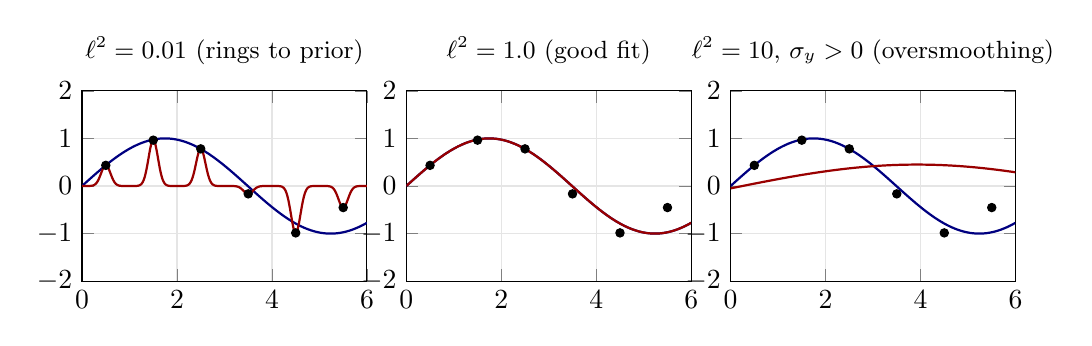
\begin{tikzpicture}
% Panel 1: small length scale: interpolates but rings down to zero between points
\begin{axis}[
    name=plot1,
    width=5.2cm, height=4cm,
    title={\small $\ell^2 = 0.01$ (rings to prior)},
    xmin=0, xmax=6, ymin=-2, ymax=2,
    grid=major, grid style={gray!20},
    every axis plot/.append style={no markers},
]
\addplot[uzhblue, thick, domain=0:6, samples=200] {sin(deg(0.9*x))};
\addplot[harvardcrimson, thick, domain=0:6, samples=400]
    {0.434*exp(-(x-0.5)^2/0.02) + 0.963*exp(-(x-1.5)^2/0.02)
   + 0.780*exp(-(x-2.5)^2/0.02) - 0.165*exp(-(x-3.5)^2/0.02)
   - 0.985*exp(-(x-4.5)^2/0.02) - 0.453*exp(-(x-5.5)^2/0.02)};
\addplot[only marks, mark=*, mark size=1.5pt] coordinates
    {(0.5,0.434) (1.5,0.963) (2.5,0.780) (3.5,-0.165) (4.5,-0.985) (5.5,-0.453)};
\end{axis}

% Panel 2: good length scale
\begin{axis}[
    name=plot2, at={(plot1.east)}, anchor=west, xshift=0.5cm,
    width=5.2cm, height=4cm,
    title={\small $\ell^2 = 1.0$ (good fit)},
    xmin=0, xmax=6, ymin=-2, ymax=2,
    grid=major, grid style={gray!20},
    every axis plot/.append style={no markers},
]
\addplot[uzhblue, thick, domain=0:6, samples=100] {sin(deg(0.9*x))};
\addplot[harvardcrimson, thick, domain=0:6, samples=100] {sin(deg(0.9*x))};
\addplot[only marks, mark=*, mark size=1.5pt] coordinates
    {(0.5,0.434) (1.5,0.963) (2.5,0.780) (3.5,-0.165) (4.5,-0.985) (5.5,-0.453)};
\end{axis}

% Panel 3: large length scale + noise: oversmooths, doesn't interpolate
\begin{axis}[
    name=plot3, at={(plot2.east)}, anchor=west, xshift=0.5cm,
    width=5.2cm, height=4cm,
    title={\small $\ell^2 = 10$, $\sigma_y > 0$ (oversmoothing)},
    xmin=0, xmax=6, ymin=-2, ymax=2,
    grid=major, grid style={gray!20},
    every axis plot/.append style={no markers},
]
\addplot[uzhblue, thick, domain=0:6, samples=100] {sin(deg(0.9*x))};
\addplot[harvardcrimson, thick, domain=0:6, samples=100] {0.5*sin(deg(0.4*x)) - 0.05};
\addplot[only marks, mark=*, mark size=1.5pt] coordinates
    {(0.5,0.434) (1.5,0.963) (2.5,0.780) (3.5,-0.165) (4.5,-0.985) (5.5,-0.453)};
\end{axis}
\end{tikzpicture}
\end{center}

\vspace{0.2cm}
\begin{itemize}
  \item \textcolor{uzhblue}{\textbf{Blue:}} true function $f(x) = \sin(0.9x)$. \textcolor{harvardcrimson}{\textbf{Red:}} GP posterior mean.
  \item \textbf{Too small $\ell$ (noiseless):} interpolates exactly but the posterior rings back to the prior mean between points $\Rightarrow$ poor predictions away from data.
  \item \textbf{Too large $\ell$ + noise:} GP smooths through the data, misses high-frequency structure of $f$.
  \item \textbf{Bias--variance trade-off in kernel form:} short $\ell$ $\Rightarrow$ low bias but high variance and ringing; long $\ell$ plus large $\sigma_y^2$ $\Rightarrow$ high bias and oversmoothing.
\end{itemize}

$\Rightarrow$ We need a principled way to learn $\ell$, $\sigma_f^2$, and $\sigma_y^2$.
\end{frame}

% --- Slide 26: Learning Hyperparameters ---
\begin{frame}{Learning Kernel Hyperparameters}
\textbf{Problem:} How to choose $\ell$, $\sigma_f$, $\sigma_y$?  $\Rightarrow$ Maximize the \emphc{marginal likelihood}.

\vspace{0.2cm}
\begin{block}{Marginal likelihood (model evidence, zero-mean prior)}
\[
\log p(\bm{y}\,|\,\X) = \underbrace{-\tfrac{1}{2}\bm{y}^\top K_y^{-1}\bm{y}}_{\text{data fit}}
\underbrace{-\tfrac{1}{2}\log|K_y|}_{\text{complexity penalty}}
\underbrace{-\tfrac{N}{2}\log(2\pi)}_{\text{constant}}
\]
\end{block}

\vspace{0.1cm}
\begin{columns}[T]
\begin{column}{0.48\textwidth}
\textbf{Intuition:}
\begin{itemize}\setlength{\itemsep}{2pt}
  \item \textbf{Data fit} $\uparrow$: reward explaining observations
  \item \textbf{Complexity} $\downarrow$: penalize overly flexible models
  \item Balance $=$ \emphc{automatic Occam's razor}
\end{itemize}
\end{column}
\begin{column}{0.48\textwidth}
\textbf{Optimization:}
\begin{itemize}\setlength{\itemsep}{1pt}\small
  \item Gradient ascent on $\log p(\bm{y}|\X)$
  \item Kernel HPs $\theta_{\mathrm{GP}}\!=\!\{\ell, \sigma_f, \sigma_y\}$ (separate from structural $\theta$ and NN $\theta_{NN}$)
  \item Closed-form gradients
  \item scikit-learn, GPyTorch
\end{itemize}
\end{column}
\end{columns}
\end{frame}

% --- New slide: Leave-one-out predictive error ---
\begin{frame}{Leave-One-Out Predictive Error}
\textbf{Idea.} Out-of-sample predictive accuracy without holding out data.

\smallskip
For a GP on $\{(\x_i, y_i)\}_{i=1}^n$ with noise $\sigma_y^2$:
\begin{equation*}
\mu_{-i}(\x_i) - y_i \;=\; -\frac{[K_y^{-1}\bm y]_i}{[K_y^{-1}]_{ii}}, \qquad
\sigma_{-i}^2(\x_i) \;=\; \frac{1}{[K_y^{-1}]_{ii}}.
\end{equation*}

\smallskip
\textbf{Why free.} Once $\mathrm{diag}(K_y^{-1})$ and $K_y^{-1}\bm y$ are available from the same Cholesky factor used for posterior inference, all $n$ LOO residuals cost only $\mathcal O(n)$ extra. No re-training, no held-out split lost.

\smallskip
\textbf{Use cases.} Surrogate-health diagnostic across active-learning rounds in SMM.

\medskip
{\scriptsize Closed form: Rasmussen \& Williams (2006), \S5.4.2.}
\end{frame}

% --- Slide 27: GPR Example Code ---
\begin{frame}[fragile]{GPR: Numpy Implementation Sketch}
\begin{lstlisting}[basicstyle=\footnotesize\ttfamily]
import numpy as np
from scipy.linalg import cho_factor, cho_solve

def kernel(X1, X2, l=1.0, sf=1.0):
    sq = np.sum(X1**2,1).reshape(-1,1) \
         + np.sum(X2**2,1) - 2*X1@X2.T
    return sf**2 * np.exp(-0.5 * sq / l**2)

K = kernel(X_tr, X_tr) + 1e-8*np.eye(N)
L, low = cho_factor(K, lower=True)  # Cholesky
alpha = cho_solve((L, low), y_tr)   # weights

Ks = kernel(X_tr, X_te)
mu  = Ks.T @ alpha                  # mean
v   = cho_solve((L, low), Ks)
var = kernel(X_te, X_te) - Ks.T @ v # variance
\end{lstlisting}

{\scriptsize See \textbf{Algorithm 2.1} in Rasmussen \& Williams (2006), and notebook \texttt{05\_GP\_and\_BAL.ipynb}.}
\end{frame}

% --- Slide 28: GP in Practice ---
\begin{frame}{GP in Practice: scikit-learn \& GPyTorch}
\begin{columns}[T]
\begin{column}{0.48\textwidth}
\textbf{scikit-learn:}
\begin{itemize}
  \item \texttt{GaussianProcessRegressor}
  \item Automatic hyperparameter tuning via marginal likelihood
  \item Great for prototyping ($N \leq 10^4$)
  \item CPU only
\end{itemize}
\end{column}
\begin{column}{0.48\textwidth}
\textbf{GPyTorch:}
\begin{itemize}
  \item GPU-accelerated GP inference
  \item Scalable to $N > 10^5$ (inducing points, KISS-GP)
  \item Integrates with PyTorch ecosystem
  \item Production-ready
\end{itemize}
\end{column}
\end{columns}

\vspace{0.5cm}
\begin{block}{Hands-on}
\textbf{Notebook:} \texttt{05\_GP\_and\_BAL.ipynb} --- GP regression from scratch, scikit-learn, and Bayesian Active Learning.
\end{block}
\end{frame}

% --- Slide 29: Prediction and Confidence Intervals ---
\begin{frame}[shrink=5]{Prediction \& Confidence Intervals}
\begin{center}
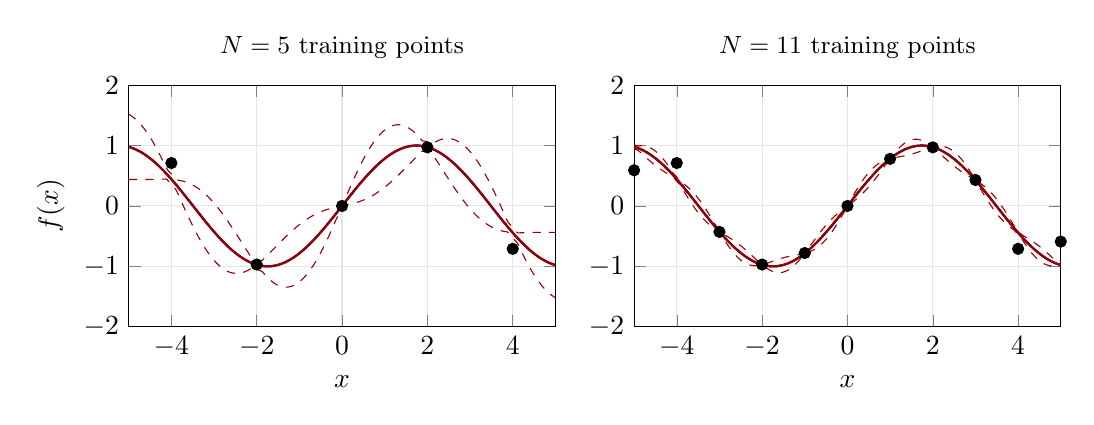
\begin{tikzpicture}
% Left panel: 5 widely-spaced training points -- CI shrinks at data, balloons between
\begin{axis}[
    name=left,
    width=7cm, height=4.65cm,
    title={\small $N = 5$ training points},
    xlabel={$x$}, ylabel={$f(x)$},
    xmin=-5, xmax=5, ymin=-2, ymax=2,
    grid=major, grid style={gray!20},
    every axis plot/.append style={no markers},
]
\addplot[uzhblue, thick, domain=-5:5, samples=200] {sin(deg(0.9*x))};
\addplot[harvardcrimson, thick, domain=-5:5, samples=200] {sin(deg(0.9*x))};
% CI envelope: shrinks near each training point (5 nearest-neighbor Gaussian "wells").
\addplot[harvardcrimson, thin, dashed, domain=-5:5, samples=400]
    {sin(deg(0.9*x)) + 0.6*sqrt( max(1 - exp(-(x+4)^2/0.6) - exp(-(x+2)^2/0.6) - exp(-(x-0)^2/0.6) - exp(-(x-2)^2/0.6) - exp(-(x-4)^2/0.6), 0.02) )};
\addplot[harvardcrimson, thin, dashed, domain=-5:5, samples=400]
    {sin(deg(0.9*x)) - 0.6*sqrt( max(1 - exp(-(x+4)^2/0.6) - exp(-(x+2)^2/0.6) - exp(-(x-0)^2/0.6) - exp(-(x-2)^2/0.6) - exp(-(x-4)^2/0.6), 0.02) )};
\addplot[only marks, mark=*, mark size=2pt, black] coordinates
    {(-4,0.71) (-2,-0.97) (0,0) (2,0.97) (4,-0.71)};
\end{axis}

% Right panel: 11 closely-spaced training points -- band is uniformly tight
\begin{axis}[
    at={(left.east)}, anchor=west, xshift=1cm,
    width=7cm, height=4.65cm,
    title={\small $N = 11$ training points},
    xlabel={$x$},
    xmin=-5, xmax=5, ymin=-2, ymax=2,
    grid=major, grid style={gray!20},
    every axis plot/.append style={no markers},
]
\addplot[uzhblue, thick, domain=-5:5, samples=200] {sin(deg(0.9*x))};
\addplot[harvardcrimson, thick, domain=-5:5, samples=200] {sin(deg(0.9*x))};
\addplot[harvardcrimson, thin, dashed, domain=-5:5, samples=400]
    {sin(deg(0.9*x)) + 0.15*sqrt( max(1 - exp(-(x+5)^2/0.15) - exp(-(x+4)^2/0.15) - exp(-(x+3)^2/0.15) - exp(-(x+2)^2/0.15) - exp(-(x+1)^2/0.15) - exp(-x^2/0.15) - exp(-(x-1)^2/0.15) - exp(-(x-2)^2/0.15) - exp(-(x-3)^2/0.15) - exp(-(x-4)^2/0.15) - exp(-(x-5)^2/0.15), 0.05) )};
\addplot[harvardcrimson, thin, dashed, domain=-5:5, samples=400]
    {sin(deg(0.9*x)) - 0.15*sqrt( max(1 - exp(-(x+5)^2/0.15) - exp(-(x+4)^2/0.15) - exp(-(x+3)^2/0.15) - exp(-(x+2)^2/0.15) - exp(-(x+1)^2/0.15) - exp(-x^2/0.15) - exp(-(x-1)^2/0.15) - exp(-(x-2)^2/0.15) - exp(-(x-3)^2/0.15) - exp(-(x-4)^2/0.15) - exp(-(x-5)^2/0.15), 0.05) )};
\addplot[only marks, mark=*, mark size=2pt, black] coordinates
    {(-5,0.59) (-4,0.71) (-3,-0.43) (-2,-0.97) (-1,-0.78) (0,0)
     (1,0.78) (2,0.97) (3,0.43) (4,-0.71) (5,-0.59)};
\end{axis}
\end{tikzpicture}
\end{center}

\vspace{0.05cm}
{\footnotesize \textcolor{uzhblue}{\textbf{Blue:}} true function. \textcolor{harvardcrimson}{\textbf{Red:}} posterior mean. \textcolor{harvardcrimson}{\textbf{Dashed:}} approximate 95\% credible band. The band collapses at training inputs (noiseless GP) and widens between them; with more data the band stays uniformly tight.}
\end{frame}

% --- Slide 30: Algorithmic Complexity ---
\begin{frame}[shrink=5]{Algorithmic Complexity}
\begin{block}{Cost of GP inference}
\begin{itemize}
  \item \textbf{Training:} Cholesky decomposition of $K_y \in \R^{N \times N}$: \emphc{$O(N^3)$}.
  \item \textbf{Prediction (per test point, after one-off precomputation of $\bm\alpha = K_y^{-1}\bm y$):} $O(N)$ for mean, $O(N^2)$ for variance.
  \item \textbf{Hyperparameter optimization:} $O(N^3)$ per gradient step.
\end{itemize}
\end{block}

\vspace{0.15cm}
\begin{block}{Scaling strategies for large $N$}
\begin{itemize}
  \item \textbf{Sparse GPs:} Inducing point methods --- approximate $K$ with rank-$M$ matrix ($M \ll N$), cost $O(NM^2)$.
  \item \textbf{Random features:} Approximate kernel with random Fourier features.
  \item \textbf{GPyTorch:} KISS-GP, structured kernel interpolation, GPU acceleration.
\end{itemize}
\end{block}

\vspace{0.1cm}
{\footnotesize For the surrogate problems in this course ($N \leq 10^4$, $d \leq 10$), standard GPs are sufficient.}
\end{frame}

% --- Slide 31: GPs vs DNNs ---
\begin{frame}{GPs vs DNNs: When to Use Which}
\begin{center}
\footnotesize
\setlength{\tabcolsep}{4pt}
\begin{tabular}{l l l}
\toprule
\textbf{Criterion} & \textbf{Gaussian Processes} & \textbf{Deep Neural Networks} \\
\midrule
Uncertainty quantification & \textcolor{darkgreen}{Built-in (posterior variance)} & \textcolor{darkred}{Requires ensembles / MC dropout} \\
Hyperparameter tuning & \textcolor{darkgreen}{Marginal likelihood} & \textcolor{softorange}{Grid search / Bayesian opt.} \\
Scaling with $N$ & \textcolor{darkred}{$O(N^3)$, limit $\sim 10^4$} & \textcolor{darkgreen}{$O(N)$ per epoch} \\
Scaling with $d$ & \textcolor{darkred}{Curse of dimensionality} & \textcolor{darkgreen}{Handles $d \gg 100$} \\
Small data ($N < 100$) & \textcolor{darkgreen}{Excellent} & \textcolor{darkred}{Typically underfits} \\
Training & \textcolor{darkgreen}{Closed-form} & \textcolor{softorange}{SGD, many epochs} \\
Interpretability & \textcolor{darkgreen}{Kernel encodes prior} & \textcolor{darkred}{Black box} \\
\bottomrule
\end{tabular}
\end{center}

\vspace{0.3cm}
\begin{alertblock}{Rule of thumb}
{\small
\begin{itemize}\itemsep0pt
  \item \textbf{$d \leq 10$, need UQ:} GPs (+ BAL).
  \item \textbf{$d > 10$, large data:} DNNs.
\end{itemize}}
\end{alertblock}
\end{frame}

% --- Slide 31b: Deep Kernel Learning ---
\begin{frame}{Deep Kernel Learning: Neural Features + GP Uncertainty}
\small
\begin{columns}[T]
\begin{column}{0.54\textwidth}
\textbf{Idea:} learn a feature map $\phi_{\theta}(\x)$ with a neural network, then use
\[
\textstyle k_{\text{DKL}}(\x,\x') = k_{\text{base}}\bigl(\phi_{\theta}(\x), \phi_{\theta}(\x')\bigr)
\]
so the GP operates in the learned feature space.

\vspace{0.05cm}
\begin{itemize}\itemsep0.1em
  \item \textbf{Front end:} the DNN learns a geometry where the target is smoother.
  \item \textbf{Back end:} the GP still provides posterior mean and variance.
  \item \textbf{Training:} optimize the feature map and kernel hyperparameters via the GP marginal likelihood.
\end{itemize}

\end{column}

\begin{column}{0.42\textwidth}
\begin{center}
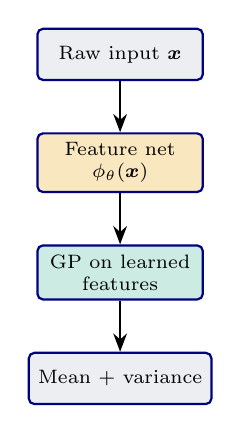
\begin{tikzpicture}[
    box/.style={rectangle, draw=uzhblue, fill=uzhgreylight, rounded corners=2pt,
        minimum width=2.1cm, minimum height=0.65cm, align=center, font=\scriptsize, thick},
    >=Stealth
]
\node[box] (raw) {Raw input $\x$};
\node[box, below=0.65cm of raw, fill=softorange!25] (net) {Feature net\\$\phi_{\theta}(\x)$};
\node[box, below=0.65cm of net, fill=softgreen!20] (gp) {GP on learned\\features};
\node[box, below=0.65cm of gp] (out) {Mean + variance};
\draw[->, thick] (raw) -- (net);
\draw[->, thick] (net) -- (gp);
\draw[->, thick] (gp) -- (out);
\end{tikzpicture}
\end{center}
\end{column}
\end{columns}
\end{frame}

% --- Slide 31c: When DKL Helps ---
\begin{frame}[shrink=20]{When Do Deep Kernels Help?}
\begin{columns}[T]
\begin{column}{0.52\textwidth}
\textbf{Standard GP assumption:} Euclidean distance in the \emph{raw input space} is informative.

\vspace{0.2cm}
\textbf{Failure modes:}
\begin{itemize}
  \item Hidden regimes / thresholds / nonstationarity
  \item Inputs are badly warped coordinates of a simple latent state
  \item Moderate-to-high-dimensional raw features with strong correlations
  \item You still need \emphc{uncertainty quantification} or BAL
\end{itemize}
\end{column}

\begin{column}{0.43\textwidth}
\begin{alertblock}{Rule of thumb}
\begin{itemize}
  \item If the input is already low-dimensional and smooth: \textbf{plain GP} is usually enough.
  \item If the latent structure is smooth but the raw geometry is poor: \textbf{DKL} is often the right bridge.
  \item If $d$ is huge and UQ is not central: \textbf{pure DNN surrogate}.
\end{itemize}
\end{alertblock}
\end{column}
\end{columns}

\vspace{0.2cm}
{\small In short: \emphc{DKL answers the question ``Can we combine DNN feature learning with GP uncertainty?''}}

\vspace{0.05em}
{\scriptsize\emph{Note on the companion notebook (NB~08).}  The DKL implementation in NB~08 trains the feature extractor against a hand-crafted teacher feature map for didactic clarity, not jointly with the GP marginal likelihood; see GPyTorch's \texttt{DeepKernel} for the joint form.}
\end{frame}

% --- Summary: Appendix A ---
\begin{frame}{Summary: Gaussian Process Regression}
\begin{enumerate}
  \item \textbf{GPs} = nonparametric Bayesian regression with \emphc{built-in UQ}.
  \item \textbf{Kernel} encodes prior beliefs (smoothness, scale, periodicity).
  \item \textbf{Posterior:} closed-form mean and variance, conditioned on data.
  \item \textbf{Hyperparameters:} learned by maximizing the marginal likelihood (automatic Occam's razor).
  \item \textbf{Limitation:} $O(N^3)$ scaling; best for moderate $N$ and $d$.
  \item \textbf{DKL:} neural feature extractor + GP head = useful when raw inputs are warped or moderately high-dimensional, but you still want UQ.
\end{enumerate}

\vspace{0.3cm}
\textbf{Next:} Use the GP's uncertainty to \emphc{intelligently select training points} --- Bayesian Active Learning.
\end{frame}

% ============================================================================
% APPENDIX B: BAYESIAN ACTIVE LEARNING
% ============================================================================
\section{Appendix B: Bayesian Active Learning}

% --- Slide 33: Motivation ---
\begin{frame}{Motivation: Where to Sample?}
\begin{columns}[T]
\begin{column}{0.48\textwidth}
\textbf{Uniform sampling:}
\begin{itemize}
  \item Places points evenly across the domain
  \item Wastes evaluations in smooth regions
  \item Cannot adapt to function complexity
\end{itemize}
\end{column}
\begin{column}{0.48\textwidth}
\textbf{Adaptive / active sampling:}
\begin{itemize}
  \item Concentrates points where the function is \emphc{hard to approximate}
  \item Uses the model's \emphc{uncertainty} to guide selection
  \item Fewer evaluations for the same accuracy
\end{itemize}
\end{column}
\end{columns}

\vspace{0.5cm}
\begin{alertblock}{Key question}
Given a budget of $N$ model evaluations, which input points $\{x_1, \dots, x_N\}$ minimize the overall approximation error?
\end{alertblock}
\end{frame}

% --- Slide 34: BAL — The Idea ---
\begin{frame}{Bayesian Active Learning: The Idea}
\textbf{Use the GP posterior variance to guide sampling.}

\vspace{0.2cm}
\begin{block}{A general score function}
\vspace{-4pt}
\[
U(\x) = w_{\mathrm{obj}} \cdot \mu(\x) + \frac{w_{\mathrm{var}}}{2}\log\sigma^2(\x)
\]
\vspace{-8pt}
\begin{itemize}\setlength{\itemsep}{1pt}\small
  \item $\sigma^2(\x)$: posterior variance \,---\, \emphc{exploration}; sampling where large reduces global uncertainty.
  \item $\mu(\x)$: posterior mean \,---\, \emphc{objective-following} bias (useful in Bayesian optimisation, not for global surrogate accuracy).
  \item $w_{\mathrm{obj}}, w_{\mathrm{var}} \geq 0$: fixed weights.
\end{itemize}
\end{block}

\vspace{0.1cm}
{\small\textbf{Default:} pure exploration ($w_{\mathrm{obj}} = 0$, maximise $\sigma^2$, i.e.\ uncertainty sampling) for surrogate building. Add the $\mu$-term when also targeting an optimum.}
\end{frame}

% --- Slide 35: BAL Algorithm ---
\begin{frame}{BAL Algorithm}
\begin{algorithm}[H]
\caption{Bayesian Active Learning for Surrogates}
\begin{algorithmic}[1]
\REQUIRE Initial design $\mathcal{D}_0 = \{(\x_i, y_i)\}_{i=1}^{n_0}$, budget $N$, candidate set $\mathcal{C}$
\STATE Fit GP on $\mathcal{D}_0$: compute posterior mean $\mu(\cdot)$ and variance $\sigma^2(\cdot)$
\FOR{$t = 1, \dots, N - n_0$}
    \STATE Compute score $U(\x) = w_{\mathrm{obj}}\,\mu(\x) + \frac{w_{\mathrm{var}}}{2}\log\sigma^2(\x)$ for all $\x \in \mathcal{C}$
    \STATE Select $\x_{\text{new}} = \argmax_{\x \in \mathcal{C}} U(\x)$
    \STATE Query the expensive model: $y_{\text{new}} = f(\x_{\text{new}})$
    \STATE Update: $\mathcal{D}_t \leftarrow \mathcal{D}_{t-1} \cup \{(\x_{\text{new}}, y_{\text{new}})\}$
    \STATE Refit GP on $\mathcal{D}_t$
\ENDFOR
\RETURN Trained GP surrogate
\end{algorithmic}
\end{algorithm}
\end{frame}

% --- Slide: BAL in Action ---
\begin{frame}{BAL in Action: Progressive Refinement}
{\small BAL selects each new point where the \emphc{posterior variance is largest} (green diamond), causing the credible band to shrink exactly where it was widest.}

\vspace{-0.05cm}
\begin{center}
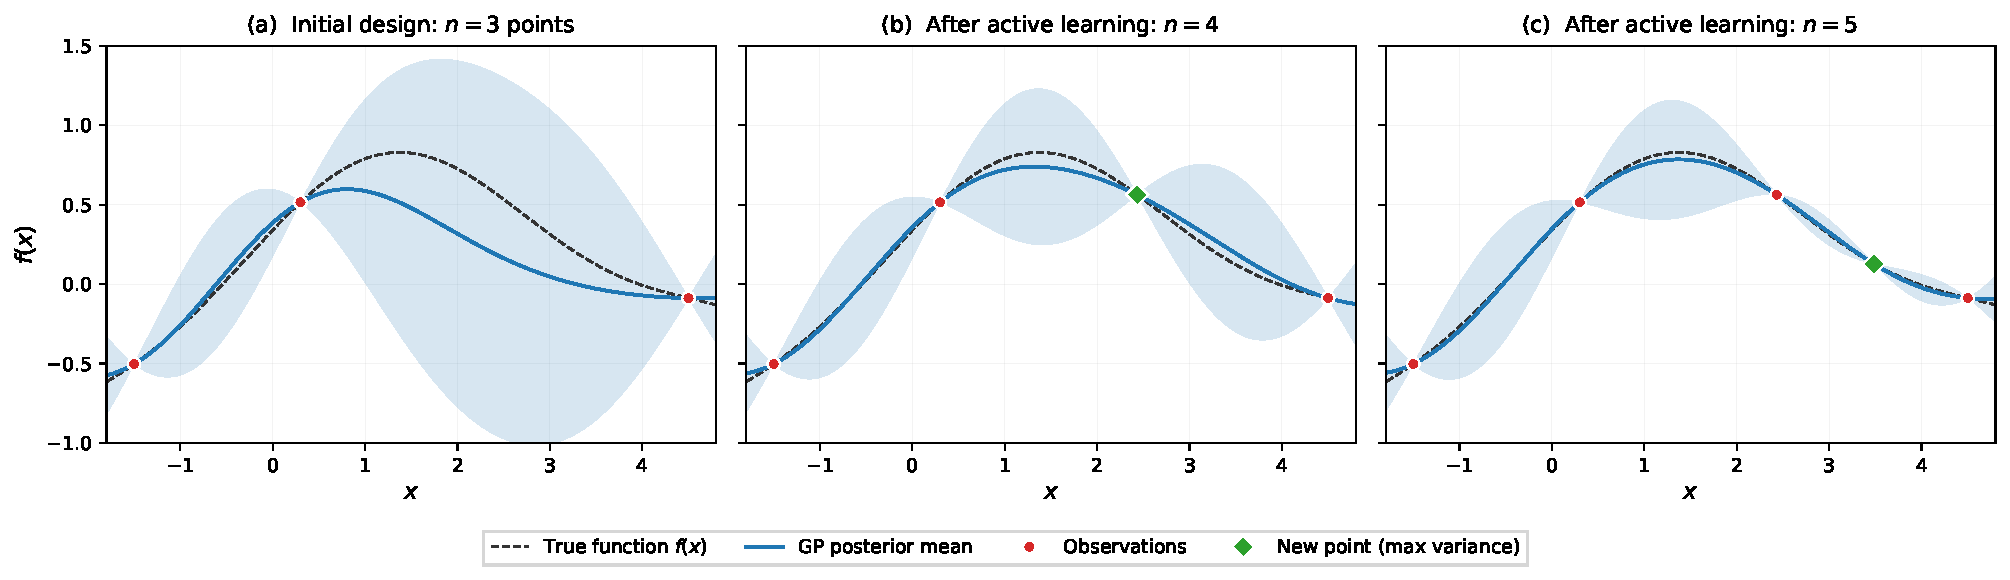
\includegraphics[width=0.95\textwidth]{fig/gp_active_learning.pdf}
\end{center}

\vspace{-0.3cm}
{\footnotesize
\begin{itemize}\setlength{\itemsep}{0pt}\setlength{\parskip}{0pt}
  \item[\textbf{(a)}] 3 initial observations (red dots); GP posterior (blue) deviates in data-sparse regions with wide 95\% CI.
  \item[\textbf{(b)}] Acquisition function picks max-variance point (green diamond); posterior tightens locally.
  \item[\textbf{(c)}] Second iteration fills the remaining gap --- 5 points suffice to track the true function.
\end{itemize}
\vspace{-0.15cm}
\textbf{Key contrast with uniform:} BAL concentrates points where the function is hardest to approximate.\\[2pt]
\emph{(Pre-generated illustration; notebook \texttt{05\_GP\_and\_BAL.ipynb} reproduces the BAL loop itself.)}}
\end{frame}

% --- Slide 38: Applications in Economics ---
\begin{frame}{BAL in Economics}
\begin{columns}[T]
\begin{column}{0.48\textwidth}
\begin{block}{Grid-free approximation}
BAL + GP $=$ grid-free adaptive sparse grids:
\begin{itemize}\setlength{\itemsep}{1pt}
  \item No structured grid needed
  \item Refinement via posterior variance
  \item Scales to $d \leq 10$
\end{itemize}
\end{block}
\end{column}
\begin{column}{0.48\textwidth}
\begin{block}{Applications}
\begin{itemize}\setlength{\itemsep}{1pt}
  \item \textbf{Optimal carbon tax}
  \item \textbf{Dynamic incentives} (kinks)
  \item \textbf{Asset pricing} (moderate $d$)
\end{itemize}
\end{block}
\end{column}
\end{columns}

\vspace{0.3cm}
{\small References: Renner \& Scheidegger (2018); K\"ubler, Scheidegger \& Surbek (2026, forthcoming in \emph{JPE Macroeconomics}).}
\end{frame}

% --- Slide 39: BAL + GP for Surrogates ---
\begin{frame}[shrink=5]{Combining BAL and GP for Surrogates}
\begin{center}
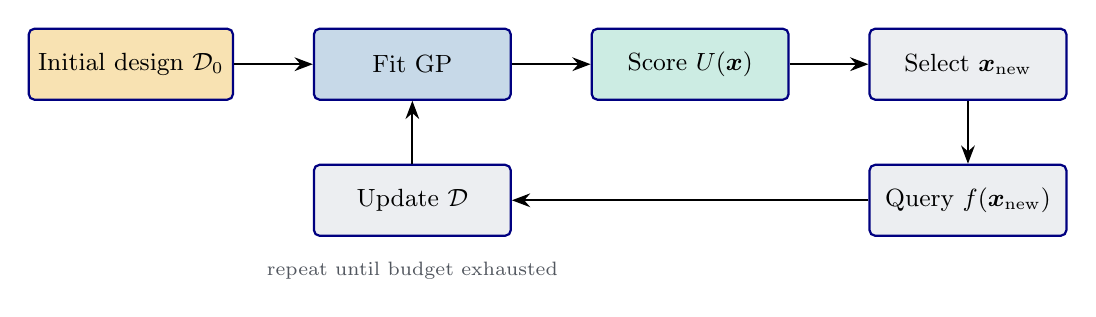
\begin{tikzpicture}[
    mlstep/.style={rectangle, draw=uzhblue, fill=uzhgreylight,
        minimum width=2.5cm, minimum height=0.9cm, font=\small,
        rounded corners=2pt, thick},
    >=Stealth
]
\node[mlstep, fill=softorange!30] (init) {Initial design $\mathcal{D}_0$};
\node[mlstep, right=1cm of init, fill=softblue!30] (gp) {Fit GP};
\node[mlstep, right=1cm of gp, fill=softgreen!20] (score) {Score $U(\x)$};
\node[mlstep, right=1cm of score] (select) {Select $\x_{\text{new}}$};
\node[mlstep, below=0.8cm of select] (query) {Query $f(\x_{\text{new}})$};
\node[mlstep, below=0.8cm of gp] (update) {Update $\mathcal{D}$};

\draw[->, thick] (init) -- (gp);
\draw[->, thick] (gp) -- (score);
\draw[->, thick] (score) -- (select);
\draw[->, thick] (select) -- (query);
\draw[->, thick] (query) -- (update);
\draw[->, thick] (update) -- (gp);

\node[below=0.2cm of update, font=\scriptsize, text=uzhgreydark] {repeat until budget exhausted};
\end{tikzpicture}
\end{center}

\vspace{0.3cm}
\begin{block}{Why this combination works}
\begin{itemize}
  \item \textbf{GP provides UQ:} posterior variance tells us where the approximation is uncertain.
  \item \textbf{BAL selects training points:} maximize information gain per model evaluation.
  \item \textbf{Surrogate = trained GP:} the same GP used for selection serves as the surrogate.
\end{itemize}
\end{block}

{\small Ideal for $d \leq 10$ when each model evaluation costs minutes to hours.}
\end{frame}

% --- Summary: Appendix B ---
\begin{frame}{Summary: Bayesian Active Learning}
\begin{enumerate}
  \item \textbf{BAL} = principled data selection using GP uncertainty.
  \item \textbf{Score function} balances exploration (high $\sigma^2$) and exploitation (high $\mu$).
  \item \textbf{Faster convergence} than uniform sampling, especially for functions with kinks or local features.
  \item \textbf{Application:} surrogate construction for moderate-dimensional problems.
\end{enumerate}

\vspace{0.3cm}
\begin{block}{Hands-on}
\textbf{Notebook:} \texttt{05\_GP\_and\_BAL.ipynb} --- GP from scratch, scikit-learn GP, and BAL comparison.
\end{block}
\end{frame}
\section{Appendix D: Toolbox \& References}

% --- Slide: Toolbox Recap ---
\begin{frame}{Recap: The Computational Toolbox}
\small
\begin{columns}[T]
\begin{column}{0.24\textwidth}
\begin{block}{\small PINNs}
\scriptsize
\begin{itemize}\itemsep0pt
  \item Continuous-time PDEs
  \item Physics loss
  \item Mesh-free
  \item HJB, Black--Scholes
\end{itemize}
\end{block}
\end{column}
\begin{column}{0.24\textwidth}
\begin{block}{\small Deep Surrogates}
\scriptsize
\begin{itemize}\itemsep0pt
  \item Discrete-time
  \item Pseudo-states
  \item Fast evaluation
  \item Estimation, UQ
\end{itemize}
\end{block}
\end{column}
\begin{column}{0.24\textwidth}
\begin{block}{\small GPs + BAL}
\scriptsize
\begin{itemize}\itemsep0pt
  \item Nonparametric
  \item Built-in UQ
  \item Active learning
  \item Moderate dim
\end{itemize}
\end{block}
\end{column}
\end{columns}

\vspace{0.3cm}
All three approaches are \emphc{complementary}: choose based on the problem structure, dimensionality, whether UQ is needed, and available hardware.\\[2pt]
{\scriptsize PINNs are not covered in this school; see the lecture script for a primer.}
\end{frame}

% --- Slide 42: The Toolbox ---
\begin{frame}{The Toolbox: When to Use What}
\begin{center}
\scriptsize
\begin{tabular}{l l l}
\toprule
\textbf{Method} & \textbf{Best for} & \textbf{Key strength} \\
\midrule
\textbf{DEQN} & Discrete-time equilibrium models & Scales to high $d$, Euler eq.\ loss \\
\textbf{PINN} & Continuous-time PDEs/HJB & Mesh-free, physics-constrained \\
\textbf{Deep Surrogate} & Fast evaluation, estimation, UQ & Pseudo-states, autograd \\
\textbf{GP + BAL} & Moderate $d$, need UQ & Built-in uncertainty, active learning \\
\textbf{Deep Kernel} & Warped inputs + need UQ & Learned features + GP uncertainty \\
\bottomrule
\end{tabular}
\end{center}

\vspace{0.15cm}
\begin{block}{Decision heuristic}
\scriptsize
\begin{enumerate}
  \item Is it a continuous-time PDE? $\Rightarrow$ \textbf{PINN}.
  \item Do you need to re-evaluate for many parameter values? $\Rightarrow$ \textbf{Deep Surrogate}.
  \item Is $d \leq 10$ and you need UQ / active learning? $\Rightarrow$ \textbf{GP + BAL}.
  \item Is the latent structure smooth, but the raw input geometry is poor? $\Rightarrow$ \textbf{Deep Kernel}.
  \item Is it a discrete-time equilibrium model? $\Rightarrow$ \textbf{DEQN}.
\end{enumerate}
\end{block}
\end{frame}

% --- Slide 43: References & Questions ---
\begin{frame}[shrink=5]{References \& Resources}
\footnotesize
\textbf{Key papers:}
\begin{itemize}\itemsep0pt \parskip0pt
  \item Chen, Didisheim \& Scheidegger (2026). \emph{Deep Surrogates for Finance: With an Application to Option Pricing.} J.\ Financial Econ.
  \item Scheidegger \& Bilionis (2019). \emph{ML for High-Dim Dynamic Stochastic Economies.} J.\ Comput.\ Sci.
  \item K\"ubler, Scheidegger \& Surbek (2026). \emph{Using Machine Learning to Compute Constrained Optimal Carbon Tax Rules.} Forthcoming in \emph{JPE Macroeconomics}.
  \item Rasmussen \& Williams (2006). \emph{GP for ML.} MIT Press.
  \item Wilson et al.\ (2016). \emph{Deep Kernel Learning.} AISTATS.
\end{itemize}

\vspace{0.1cm}
{\tiny \textbf{Notebooks} (in \texttt{lectures/lecture\_2/code/}): \texttt{04\_Surrogate\_Primer}, \texttt{05\_GP\_and\_BAL}, \texttt{06\_Deep\_Kernel\_Learning}.}

\vspace{0.15cm}
\textbf{GitHub:} \url{https://github.com/sischei/cemracs2026_DEQN}

\vspace{0.1cm}
{\small \textbf{Next up:} Practical Session 2 --- hands-on CDICE (notebooks \texttt{01}--\texttt{03}); then Lecture 3: optimal carbon taxation and deep UQ.}

\vspace{0.2cm}
\begin{center}
{\LARGE \emphc{Questions?}}
\end{center}
\end{frame}

\end{document}
